\documentclass[a4paper,10pt,twoside]{memoir}
% Maths symbols, equation environments and physics macros:
\usepackage{amsmath,amssymb}
\usepackage{physics}

% Graphics:
\usepackage{graphicx}

% For an mbox command that works in math mode (i.e that contains math):
\usepackage{mathtools}

% Colours:
\usepackage[table]{xcolor}
\definecolor{pastelred}{RGB}{200,80,80}
\definecolor{pastelgreen}{RGB}{0,150,80}
\definecolor{battleshipgrey}{rgb}{0.52, 0.52, 0.51}


% Fonts:
\usepackage[
  % Uppercase Greek letters should be italic by default:
  math-style=ISO,
  % Uppercase bold symbols should also be italic unless set otherwise:
  bold-style=ISO,
  % Upright \nabla though:
  nabla=upright,
  % \mathrm,\mathit,\mathbf and operators should use the maths font, not the text font:
  mathup=sym,mathit=sym,mathbf=sym
]{unicode-math}

% Garamond for normal text:
\setmainfont[
    Mapping=tex-text,
    Contextuals=Alternate,
    Numbers={OldStyle,Proportional},
    BoldFont={GaramondPremrPro-Bd},
    ItalicFont={GaramondPremrPro-It},
    BoldItalicFont={GaramondPremrPro-BdIt}
    ]{Garamond Premier Pro}

% Monospaced font:
\setmonofont{Ubuntu Mono}

% Asana for all non-alphanumeric symbols, operators, etc:
\setmathfont{Asana Math}

% Latin Modern for integrals, sums, \nabla, and other symbold determined to be missing from Minion
% and Asana:
\setmathfont[range={\mathop,\nabla,\triangleright}]{Latin Modern Math}


% Minion pro for alphanumeric symbols, inlcuding Greek:
\setmathfont{MinionPro}[
    range={up}/{latin,Latin,num,Greek,greek},
    SizeFeatures = {
        {Size = -8.41, Font = MinionPro-Capt},
        {Size = 8.41-13.01, Font = MinionPro-Regular},
        {Size = 13.01-19.91, Font = MinionPro-Subh},
        {Size = 19.91-, Font = MinionPro-Disp}
    }]
\setmathfont{MinionPro-It}[
    range={it}/{latin,Latin,num,Greek,greek},
    SizeFeatures = {
        {Size = -8.41, Font = MinionPro-ItCapt},
        {Size = 8.41-13.01, Font = MinionPro-It},
        {Size = 13.01-19.91, Font = MinionPro-ItSubh},
        {Size = 19.91-, Font = MinionPro-ItDisp}
    }]
\setmathfont{MinionPro-Bold}[
    range={bfup}/{latin,Latin,num,Greek,greek},
    SizeFeatures = {
        {Size = -8.41, Font = MinionPro-BoldCapt},
        {Size = 8.41-13.01, Font = MinionPro-Bold},
        {Size = 13.01-19.91, Font = MinionPro-BoldSubh},
        {Size = 19.91-, Font = MinionPro-BoldDisp}
    }]
\setmathfont{MinionPro-BoldIt}[
    range={bfit}/{latin,Latin,num,Greek,greek},
    SizeFeatures = {
        {Size = -8.41, Font = MinionPro-BoldItCapt},
        {Size = 8.41-13.01, Font = MinionPro-BoldIt},
        {Size = 13.01-19.91, Font = MinionPro-BoldItSubh},
        {Size = 19.91-, Font = MinionPro-BoldItDisp}
    }]

% Use math font for blackboard bold:
\DeclareMathAlphabet{\mathbb}{U}{msb}{m}{n}

% Use swashed Minion Pro for mathcal:
% \setmathfont[range=cal,Contextuals=Swash]{MinionPro-It}

% Workaround for bug where the above commented out line doesn't work - it works in xelatex and will
% presumably be fixed for lualatex in the future. In the meantime we define a text font face that
% uses swashed Minion Pro, and redefine the \mathcal command to use it:
\newfontface\swash[Contextuals=Swash]{MinionPro-It}
\renewcommand\mathcal[1]{\mathmbox{\textrm{\swash #1}}}

% redefine \texttt to be coloured:
\renewcommand\texttt[1]{{\ttfamily\color{pastelgreen}#1}}

% Typesetting tweaks for pedants and perfectionists:
\usepackage{microtype}

% Better behaved \cite command:
\usepackage{cite}

% For calculating text sizes
\usepackage{calc}

% Allow rotating floats - useful for landscape float pages:
\usepackage{rotating}

% Make commands run at the start of a new page. Useful for changing the margins on a float page
% without having to manually start a new page and thus have the rest of the current page
% potentially blank:
\usepackage{afterpage}

% Drop caps:
\usepackage{lettrine}

% For making fake blocks of text for testing:
\usepackage{lipsum}

% For changing page margins, useful used in combination with \afterpage for a float page:
\usepackage{geometry}

% Captions on the side of figures
\usepackage{subfig}
\captionsetup*[figure]{position=top}

% Source code listings:
\usepackage{minted}
  % % A command for including Python source from a file, like: \python{myfile.py}
  % \newcommand{\python}[1]{\spacing{0.7}\inputminted[linenos, numbersep=5pt, frame=lines, framesep=2mm,fontsize=\scriptsize]{python}{#1}}

  % A command for including Python source from a file, like: \python{myfile.py}
  \newcommand{\python}[1]{\inputminted[linenos, numbersep=5pt, frame=lines, framesep=2mm,fontsize=\scriptsize]{python}{#1}}

% For verbatim text input
\usepackage{verbatim}

% For typesetting algorithms:
\usepackage{algorithm,algpseudocode,float}

% For stacking things:
\usepackage{stackengine}

% Page-breakable algorithm environment
\makeatletter
\newenvironment{breakablealgorithm}
  {% \begin{breakablealgorithm}
   \begin{center}
     \refstepcounter{algorithm}% New algorithm
     \hrule height.8pt depth0pt \kern2pt% \@fs@pre for \@fs@ruled
     \renewcommand{\caption}[2][\relax]{% Make a new \caption
       {\raggedright\textbf{\ALG@name~\thealgorithm} ##2\par}%
       \ifx\relax##1\relax % #1 is \relax
         \addcontentsline{loa}{algorithm}{\protect\numberline{\thealgorithm}##2}%
       \else % #1 is not \relax
         \addcontentsline{loa}{algorithm}{\protect\numberline{\thealgorithm}##1}%
       \fi
       \kern2pt\hrule\kern2pt
     }
  }{% \end{breakablealgorithm}
     \kern2pt\hrule\relax% \@fs@post for \@fs@ruled
   \end{center}
  }
\makeatother


% Hyperlinked references, contents:
\usepackage[bookmarksopen,
  pagebackref,
  pdfpagelayout=TwoPageRight,
  colorlinks=true,
  urlcolor=pastelred,
  citecolor=pastelred,
  filecolor=pastelred,
  linkcolor=pastelred,
  linktocpage=true]
  {hyperref}

% Hyperlinked back-references in the bibliography
\renewcommand*{\backrefalt}[4]{
  \ifnum#1=1
    [p~#2]
  \else
    [pp~#2]
  \fi
}

% Make links to figures link to the top of the figure instead of the caption
\usepackage[all]{hypcap}

% Remove need for extra pass of latex to make bookmarks:
\usepackage{bookmark}

% Links to DOIs in bibliography
\usepackage{doi}

% Provides \RaggedLeft and \RaggedRight commands for ragged text with occasional hyphenation:
\usepackage{ragged2e}

% Import hyperlinks from .pax files when including external pdfs

% Hacks to make pax work with lualatex, from
% https://tex.stackexchange.com/questions/60201/getting-pax-pdfpages-to-work-with-xelatex
\makeatletter
\let\pdfescapename=\pdf@escapename
\let\pdfstrcmp=\pdf@strcmp
\makeatother
\usepackage{pax}

% For including external PDF documents as pages in output:
\usepackage[final]{pdfpages}

% For defining abbreviations (that will be written in full their first use)
% \usepackage{glossaries}
% \glsdisablehyper
% \setacronymstyle{long-sc-short}

% For making some pages landscape in the PDF
\usepackage{pdflscape}

% For prettier tables:
\usepackage{booktabs}

% For multi-row tables:
\usepackage{hhline}
\usepackage{multirow}

% Tick and cross mark
\usepackage{pifont}% http://ctan.org/pkg/pifont
\newcommand{\cmark}{\ding{51}}%
\newcommand{\xmark}{\ding{55}}%


% This page left intentionally blank:
  \makeatletter \def\clearforchapter{
    \clearpage
    \if@twoside \ifodd\c@page\else
        \newgeometry{left=2.54cm,bottom=1.5in,right=2.54cm,top=1.5in}
        \hbox{}
        \vfill
        \begin{center}This page intentionally left blank
        \end{center}
        \vfill
        \thispagestyle{cleared}
        \restoregeometry%
  \newpage\if@twocolumn\hbox{}\newpage\fi\fi\fi}\makeatother

  \newcommand*{\blankpage}{%
  \newgeometry{left=2.54cm,bottom=1.5in,right=2.54cm,top=1.5in}
  \vspace*{\fill}
  \centering This page intentionally left blank
  \vspace{\fill}
  \restoregeometry}
  \makeatletter
  \renewcommand*{\cleardoublepage}{\clearpage\if@twoside \ifodd\c@page\else
  \blankpage
  \thispagestyle{empty}
  \if@twocolumn\hbox{}\newpage\fi\fi\fi}
  \makeatother


% Caption name/title style:
\captionnamefont{\normalfont\small\bfseries}
\captiontitlefont{\small\rmfamily}


%% Set contents depth and section numbering %%
\setcounter{tocdepth}{2}
\setsecnumdepth{subsection}


% Make footnotes be ragged:
\renewcommand{\foottextfont}{\footnotesize\RaggedRight}

%% Make footnotes go in the margin %%
\footnotesinmargin
\setlength{\footmarkwidth}{0em}
\setlength{\footmarksep}{0em}
\setlength{\footparindent}{0em}


% Chapter style:
\makechapterstyle{madsen_mod}{% requires graphicx package
  \chapterstyle{default}
  \renewcommand*{\chapnamefont}{%
    \normalfont\Large\scshape\raggedleft}
  \renewcommand*{\chaptitlefont}{%
    \normalfont\Huge\bfseries\raggedleft}
  \renewcommand*{\chapternamenum}{}
  \renewcommand*{\printchapternum}{%
    \makebox[0pt][l]{\hspace{0.4em}%
      \resizebox{!}{6ex}{%
        \chapnamefont\bfseries\rmfamily\color{battleshipgrey}\thechapter}%
    }%
  }%
  \renewcommand*{\printchapternonum}{%
    \chapnamefont \phantom{\printchaptername \chapternamenum%
      \makebox[0pt][l]{\hspace{0.4em}%
        \resizebox{!}{6ex}{%
          \chapnamefont\bfseries 1}%
      }%
    }%
    \afterchapternum %
  }%
  \renewcommand*{\afterchapternum}{%
    \par\hspace{1.5cm}\hrule\vskip\midchapskip}}
\chapterstyle{madsen_mod}


%% Make page headers underlined and small caps %%
\makeheadrule{headings}{\textwidth}{\normalrulethickness}
\pagestyle{headings}
\renewcommand*{\memUChead}[1]{\textsc{\MakeTextLowercase{#1}}}

% Call the Bibliography section "References"
\renewcommand{\bibname}{References}

% Draft mode: Include hg info in footers:
\immediate\write18{make hglog}
\def\hginfo{\verbatiminput{hglog.txt}}
\def\draftinfo{{\small \ttfamily \bfseries \color{red} \hginfo}}
\makeevenfoot{plain}{\draftinfo}{\thepage}{}
\makeoddfoot{plain}{\draftinfo}{\thepage}{}
\makeevenfoot{headings}{\draftinfo}{}{}
\makeoddfoot{headings}{\draftinfo}{}{}


% Page margins:
\settrims{0pt}{0pt}
\settypeblocksize{220.8mm}{4.5in}{*}
\setlrmargins{25.4mm}{*}{*}
\setulmargins{1.5in}{*}{*}
\setmarginnotes{5mm}{40mm}{\onelineskip}
\setheadfoot{\onelineskip}{2\onelineskip}
\setheaderspaces{*}{2\onelineskip}{*}
\checkandfixthelayout

% Skew accents that go over characters to make them more centered:

% \hat:
\let\oldhat\hat
\renewcommand{\hat}[1]{\skew{1.5}\oldhat{\mathmbox{#1}}}

% \tilde:
\let\oldtilde\tilde
\renewcommand{\tilde}[1]{\skew{1.5}\oldtilde{\mathmbox{#1}}}

% \dot:
\let\olddot\dot
\renewcommand{\dot}[1]{\skew{1.5}\olddot{\mathmbox{#1}}}

% \vec: Bold vector. Italic or not depending on unicode-math options.
\renewcommand{\vec}[1]{\symbf{#1}}

% Bras, kets, brakets, ketbras, expectation values, and matrix elements. Versions that don't resize
% start with a lowercase letter, versions that will resize start with uppercase letter:

\let\oldabs\abs
\renewcommand\abs[1]{\oldabs*{#1}}
\newcommand\Abs[1]{\oldabs{#1}}

\let\oldbra\bra
\renewcommand\bra[1]{\oldbra*{#1}}
\newcommand\Bra[1]{\oldbra{#1}}

\let\oldket\ket
\renewcommand\ket[1]{\oldket*{#1}}
\newcommand\Ket[1]{\oldket{#1}}

\let\oldbraket\braket
\renewcommand\braket[2]{\oldbraket*{#1}{#2}}
\newcommand\Braket[2]{\oldbraket{#1}{#2}}

\let\oldketbra\ketbra
\renewcommand\ketbra[2]{\oldketbra*{#1}{#2}}
\newcommand\Ketbra[2]{\oldketbra{#1}{#2}}

\let\oldev\ev
\renewcommand\ev[1]{\oldev*{#1}}
\newcommand\Ev[1]{\oldev{#1}}

\let\oldmatrixel\matrixel
\renewcommand\matrixel[3]{\oldmatrixel*{#1}{#2}{#3}}
\newcommand\Matrixel[3]{\oldmatrixel{#1}{#2}{#3}}

% A placeholder for zeros in matrices - a \cdot (but with a smaller command so that things are
% neater in latex source); first \makebox sets the width, second zero-width \makebox contains a
% phantom that sets the height:
\newcommand\mb{\phantom{0}}
% \newcommand\md{\makebox[0pt]{$\cdot$}\phantom{0}}
\newcommand\md{\makebox[\widthof{$0$}][c]{$\cdot$}}

% A smallmatrix with even smaller column separation:
\newenvironment{xsmallmatrix}
    {\renewcommand\thickspace{\kern1pt}\smallmatrix}
    {\endsmallmatrix}

% Imaginary and real parts as normal operators instead of script font:
\DeclareMathOperator{\im}{Im}
\DeclareMathOperator{\re}{Re}

% Sign function:
\DeclareMathOperator{\sgn}{sgn}

% Two argument arctan function:
\DeclareMathOperator{\arctantwo}{arctan2}

% Principle argument of complex number:
\DeclareMathOperator{\Arg}{Arg}
\DeclareMathOperator{\fft}{\textsc{fft}}

% % Minimum:
% \DeclareMathOperator{\min}{min}

% % Maximum:
% \DeclareMathOperator{\max}{max}

% A figref command to standardise the way figures are referenced:
\newcommand\figref[1]{Figure \ref{#1}}

% Similarly, a table command:
\newcommand\tableref[1]{Table\ref{#1}}

% Units
\newcommand\unit[1]{\,\mathrm{#1}}

% Scientific notation: times-ten-to-the
\newcommand\E[1]{\times 10^{#1}}

% \mathup in braces:
\newcommand\up[1]{{\mathup{#1}}}

% Imaginary unit, upright:
\newcommand\ii{\up{i}}

% Euler's number, upright:
\newcommand\ee{\up{e}}

% Big O notation. Choose mathscr instead of mathcal because Minion's swashed O doesn't look any different to its regular O.
\newcommand\Ord[1]{\mathscr{O}(#1)}
\newcommand\Ordx[1]{\mathscr{O}\left(#1\right)}

% A "kronecker dot product"
\newcommand\krondot{\overset{\scriptscriptstyle\otimes}\cdot}

% Overset command with small font
\newcommand\toverset[1]{\overset{\scriptscriptstyle #1}}

% Abbreviations:
% \newacronym{rk4}{rk4}{fourth order Runge--Kutta}
% \newacronym{rk4ip}{rk4ip}{fourth order Runge--Kutta in the interaction picture}
% \newacronym{rk4ilip}{rk4ilip}{fourth order Runge--Kutta in an instantaneous local interaction picture}
% \newacronym{sp}{sp}{Schr\"odinger picture}
% \newacronym{ip}{ip}{interaction picture}
% \newacronym{de}{de}{differential equation}



\newcommand\runmanager{\texttt{runmanager}}
\newcommand\labscript{\texttt{labscript}}
\newcommand\blacs{\texttt{BLACS}}
\newcommand\lyse{\texttt{lyse}}
\newcommand\bias{\texttt{BIAS}}
\newcommand\runviewer{\texttt{runviewer}}
\newcommand\bec{{\scshape bec}}
\newcommand\mot{{\scshape mot}}
\newcommand\http{{\scshape http}}
\newcommand\hdf{{\scshape hdf5}}
\newcommand\ac{{\scshape ac}}
\newcommand\rf{{\scshape rf}}
\newcommand\api{{\scshape api}}
\newcommand\dds{{\scshape dds}}

\begin{document}
\pagenumbering{gobble}
\begin{titlingpage}
\thispagestyle{empty}
\newgeometry{left=2.25in,bottom=2in,right=2.25in,top=2.5in}
\begin{centering}
\rule{\textwidth}{1pt}\par
\vspace{0.5\baselineskip}
{\HUGE\scshape State-dependent forces in \\ cold quantum gases\\}
\vspace{\baselineskip}
\rule{\textwidth}{1pt}\par
\vfill
{\Huge Christopher Billington}\\
\vfill
\Large Submitted in total fulfilment of the requirements\\
of the degree of Doctor of Philosophy\\
\vspace{\baselineskip}
\textbf{Supervisory committee:}\\
Prof~Kristian Helmerson\\
Dr~Lincoln Turner\\
Dr~Russell Anderson\\
\vfill
\begin{minipage}{3cm}
\centerfloat

\includegraphics[width=2.5cm]{figures/Monash_crest_A4.pdf}
\end{minipage}\\
{\Large School of Physics and Astronomy\\
Monash University\\
\vspace{\baselineskip}
June, 2018}\\
\end{centering}
% \draftinfo
\restoregeometry
\end{titlingpage}

\pagenumbering{roman}

\cleardoublepage

\vspace*{\fill}

\begin{center}
\begin{minipage}{0.95\textwidth}

\begin{center}
\textit{Copyright Notices}
\end{center}

{\textit{Notice 1}}

Under the Copyright Act 1968, this thesis must be used only under the normal conditions of scholarly fair dealing.
In particular no results or conclusions should be extracted from it, nor should it be copied or closely paraphrased in whole or in part without the written consent of the author.
Proper written acknowledgement should be made for any assistance obtained from this thesis.

\bigskip

{\textit {Notice 2}}

I certify that I have made all reasonable efforts to secure copyright permissions for third-party content included in this thesis and have not knowingly added copyright content to my work without the owner's permission.

\end{minipage}
\end{center}

\vspace*{\fill}
\vspace*{\fill}

\chapter*{Abstract}

% [TODO write the abstract]

\chapter*{Declaration}

This thesis contains no material that has been accepted for the award of any other degree or diploma in any university or other institution. To the best of my knowledge the thesis contains no material previously published or written by another person, except where due reference is made in the text of the thesis. For parts of this thesis that are based on joint research or publications, the relative contributions of the respective authors are detailed appropriately.

\begin{center}
\vspace{1.5cm}
\rule{8cm}{1pt}\\
\raisebox{0.5cm}[0pt][0pt]{\includegraphics[scale=0.1]{submission/cjb}}\\
Christopher Billington

\vspace{1.5cm}
\rule{8cm}{1pt}\\
\raisebox{0.5cm}[0pt][0pt]{\includegraphics[scale=0.15]{submission/kh}}\\
Professor Kristian Helmerson  

\vspace{1.5cm}
\rule{8cm}{1pt}\\
\raisebox{0.6cm}[0pt][0pt]{\includegraphics[scale=0.9]{submission/ldt}}\\
Dr Lincoln Turner

\vspace{1.5cm}
\rule{8cm}{1pt}\\
\raisebox{0.5cm}[0pt][0pt]{\includegraphics[scale=0.1]{submission/rpa}}\\
Dr Russell Anderson 

\end{center}

\chapter*{Acknowledgements}

% Over the past few years during my PhD, I've been able to learn fascinating things from interesting people, play with fun technological toys, and contribute meaningfully to scientific progress. I could not have done any of this without the support, friendship, and mentorship of many people. The Science Advanced cohort w Lincoln Turner brought me up to speed on a wide range of topics

\cleardoublepage

\tableofcontents
% \listoffigures
% \listoftables
\cleardoublepage
\pagenumbering{arabic}


% \section*{Todo list}
% \begin{itemize}
%     \item short caption for all figures for figure list and same for table list.
%     \item check for square bracketed todos
%     \item put the old what's new bits in the separate chapters
%     \item add to numerics intro mention of the fact that I use these methods in other sections. "review" "Appraisal" "quantitative comparison of benefits" "detailed quantitative appraisal" - most people's numerics sections are sparse - unexamined choice of methods. Defined target audience - new PhD students. Cite Tannor in the intro.  "rapid approach to understanding" for atomic physicists specifically. "Operational"
% Quote numerical recipes on the virtues of simplicity - arm long section of shelf in library got their numerics wrong
%     \item 3D, 2D, \textsc{2d} etc.

% \end{itemize}

% software additions:
% add figures from transfer report and from rottnest talk.
% add experiment script from transfer report - port it to new labscript.
% change titles to be the same as transfer report?

\chapter{Introduction}\label{chap:introduction}

\lettrine[lines=3]{T}{he subject of study} of this thesis is Bose--Einstein condensation, as well as associated experimental and theoeretical techniques and phenomena in cold atom physics. The following chapters describe my work in a cold atom research group over the past several years, pertaining to apparatus construction, experiment, theory, and software design and development. An overarching theme is \emph{state-dependent forces} on cold atoms. Selectively subjecting atoms to forces based on what state they are in is at the core of many phenomena in cold atom physics. As I go into in the following chapters, different types of state selectivity allow for cooling and imaging techniques that would otherwise not be possible, momentum state-selectivity is central to wave-mixing phenomena; and semiclassical models run into a problem when state-selective forces cannot be disregarded in determining the classical force that atoms modelled semiclasically ought to be subjected to.

Bose--Einstein condensates (\textsc{bec}s) in dilute atomic gases are superfluids that can be created in the lab at extremely low temperatures. This strange state of matter was predicted in 1925 by Bose and Einstein \cite{bose_plancks_1924, einstein_quantentheorie_1925} , first produced experimentally in 1995 \cite{anderson_observation_1995} in a cloud of rubidium atoms, and has since been made out of many other atoms, usually alkali metals \cite{davis_bose-einstein_1995, modugno_bose-einstein_2001, bradley_bose-einstein_1997, weber_bose-einstein_2003}. In a \textsc{bec}, a macroscopic sample of bosonic atoms all occupy the same quantum state, and many of the features of the single particle wavefunctions are exhibited by the cloud as a whole. Bose--Einstein condensation and cold atoms and ions more generally have rich applications in precision measurement \cite{robins_atom_2013, cronin_optics_2009}, quantum computation \cite{ladd_quantum_2010, negretti_quantum_2011} and quantum simulation \cite{bloch_quantum_2012, blatt_quantum_2012}.  

\section{Chapter overview}

Various experimental techniques are used to produce and study Bose--Einstein condensates, many of which exploit of necessitate an understanding of the quantum behaviour of the atomic systems in question. I summarise some of these techniques and detail the atomic physics principles underlying them in chapter \ref{chap:atomic_physics}.

The fields of Bose--Einstein condensation and cold atoms more generally enjoy a tight coupling between theory and experiment, not least because of the enduring usefulness and accuracy of mean-field theory. In mean-field theory, the quantum matter field operator of the atoms comprising a Bose--Einstein condensate is replaced with its expectation value at each point in space, allowing the entire multi-particle system to be modelled with little more computational complexity than that required to model a single-particle wavefunction.\footnote{Mean field theory is accurate in the low-temperature limit, in which it has some remaining limitations---it does not for example predict the observed $s$-wave scattering halos when two \textsc{bec} wavepackets collide \cite{norrie_quantum_2006}, but it is sufficient for modelling a  wide range of experiments nonetheless.} The resulting differential equation---the Gross--Pitaevskii equation---is nonlinear and using it to propagate a condensate wavefunction in time generally requires numerical techniques rather than analytic ones. My favourite numerical methods for doing so (which apply more generally to numerically evolving quantum systems of all kinds) are described in chapter \ref{chap:numerics}. In chapter \ref{chap:numerics} I also develop a variation on fourth-order Runge--Kutta integration which improves on one of its deficiencies for simulating quantum systems. I also present arguments that a fairly sophisticated method of discretising partial differential equations---the finite element discrete variable representation---may offer less computational efficiency that simpler methods for computing solutions of comparable accuracy to the Gross--Pitaevskii and Schr\"odinger wave equations.

As an experimental field, \textsc{bec} research involves the construction of apparatuses capable of implementing the techniques described in chapter \ref{chap:atomic_physics} in order to produce, control, and measure \textsc{bec}s. Chapter \ref{chap:experiment} describes some of the process of constructing such an apparatus, which involves a vacuum system, magnetic coils and optical systems. I present an optical layout for producing magneto-optically trapped $^{87}$Rb atoms (a step on the way to condensation) that I designed and assembled as an exchange student in the group of József Fortágh at the University of T\"ubingen's Physikalisches Institut.

Production, control, and measurement of cold atom systems require more than the necessary optics and magnetic sources to be installed---they must be controllable in a time-accurate way in order to execute the necessary cooling processes, manipulate the system as desired, and observe the results. Production of a condensate takes on the order of tens of seconds, requiring precisely timed pulses of laser light at specific frequencies, sweeps of magnetic field strengths, and frequency sweeps of radio and microwave radiation. This cannot all be done by human experimenters alone, and so requires computer automation of some kind. In chapter \ref{chap:software} I reproduce our publication on a suite of software programs, the \emph{labscript suite}. This software leverages modern software development techniques such as object orientation, abstraction and isolation as well as older principles---such as aspects of the Unix philosophy---to produce a powerful, maintainable, extensible system for designing, running and analysing shot-based experiments on commodity hardware.

As superfluids, \bec s have zero viscosity and as such can support persistent flows. In classical fluid dynamics the absence of viscosity means that a fluid cannot support vorticity,\footnote{This is because the motion of vorticity is described by a diffusion equation---with viscosity as the diffusion constant. When the diffusion constant is zero, there is no way for vorticity to enter the fluid from a boundary in the first place!} and must be irrotational. However, fluid circulation can still occur around points of zero fluid density, known as vortices. In \bec s this circulation is also quantised, in units of $h/m$.

These quantised vortices are topological defects---the phase of the macroscopic wavefunction winds by a multiple of $2\pi$ around them, and is undefined at the center of the vortex core itself.  Quantised vortices were observed in superfluid helium\footnote{In which 10\% or so of the atoms undergo Bose--Einstein condensation.} in the early 1960s \cite{vinen_detection_1961}, and in \bec\ in a dilute atomic gas in 1999 \cite{matthews_vortices_1999}. The formation, dynamics and decay of these vortices are believed to be important for the study of superfluid turbulence \cite{barenghi_quantized_2001}.

In chapter \ref{chap:velocimetry} I present simulations exploring the feasibility of imaging these vortices in-situ using \emph{tracer particles}. Atoms of one kind ($^{87}$Rb) may become trapped in the cores of quantised vortices in a condensate of another kind ($^{41}$K), and if imaged in a time-resolved way, reveal the motion of these vortices. A primary concern in any implementation of such a scheme is keeping the tracer atoms cold enough that they remain trapped in the vortex cores even as they scatter light for imaging. To that end, in chapter \ref{chap:velocimetry} I present modelling of a novel---if impractical---laser cooling scheme for Sisyphus cooling of $^{87}$Rb atoms in a $34\unit{G}$ magnetic field--- a field strength at which $^{87}$Rb and $^{41}$K repel each other strongly (leading to tighter trapping in the vortex cores).

In a \textsc{bec}, the wavelike behaviour of matter is apparent, unlike at higher temperatures at which atoms are well described as classical particles. Not only are atoms in a \textsc{bec} wavelike, they are described by a \emph{nonlinear} wave equation. As with nonlinear optical systems, they therefore exhibit wave-mixing behaviour whereby a number of momentum states may interact to produce additional momentum states. In chapter \ref{chap:wave_mixing} I describe our lab's four wave mixing experiment, which reproduced an existing result for \textsc{bec}s, and then our attempt at six wave mixing---a higher order effect (in the sense of perturbation theory). We did not observe the expected six wave mixing, rather we saw \emph{four} wave mixing despite the required resonance condition apparently being violated. This result agreed with mean-field theory  simulations however, implying that the result was unlikely to be due to some experimental error.

Atoms have spin, and when other spin-projection states cannot be disregarded, mean-field theory for spinful \textsc{bec}s takes the form of multiple, interacting fields. This allows for richer nonlinear dynamics that a single-component \textsc{bec}, with wave mixing producing new momentum states and new spin-projection states in tandem. In chapter \ref{chap:wave_mixing} I present simulation results showing this ``spin wave" mixing, although the main result is that---for $^{87}$Rb at least---the effect is very small and unlikely to be experimentally observable in existing $^{87}$Rb \textsc{bec} experiments.

As mentioned above, at high temperatures (higher than that at which atoms Bose-condense) atoms are well described as classical particles. This is true in the sense that the wavelike nature of the atoms can be disregarded---they move through space like classical billiard balls obeying Newtonian mechanics. The internal state of the atoms, however---for example the state of an outer shell electron---may not be well modelled by classical mechanics. Even at room temperature, an electron is poorly described as a classical charged particle orbiting a nucleus. When there is \emph{coupling} then, between this internal state of an atom and its motional state, the quantum-ness of the internal state can in some sense `leak' into its motional state even if the motion is otherwise modelled well classically. The classic example of this is the Stern--Gerlach experiment \cite{gerlach_experimentelle_1922}, in which a beam of atoms splits into two beams as it passes through a magnetic field gradient. A similar situation arises for atoms in a magnetic trap---a common feature of cold atom experiments and often used in the final stage of cooling to \textsc{bec}. To correctly model the losses of atoms from these traps, one needs to model the internal state of the atoms quantum-mechanically, but it is computationally expensive to also model their spatial motion using full quantum wavefunctions. We would like a way to model the atoms' motion classically, but in such a way that it can reproduce Stern--Gerlach separation---with modelled atoms taking one or the other trajectory probabilistically, with the probabilities consistent with those of a fully quantum treatment. In chapter \ref{chap:hvsc} I present such a model, one that is based on a \emph{hidden variable} carried around with each atom being modelled, which selects one of the atom's internal eigenstates. The apparent definiteness of the hidden variable allows the spatial motion part of the modelling to treat the atoms' spin projection degree of freedom as if it were in a definite state, allowing the modelling to take a single, definite trajectory. The hidden variable itself is evolved using a stochastic hidden variable theory that ensures its probability of corresponding to any particular spin-projection state is consistent with with the underlying quantum evolution of the atom's internal degrees of freedom.

\clearpage

\section{What's new in this thesis}

The following two results comprise the primary scientific contributions of this thesis:

The use of hidden variables in semiclassical models of atomic dynamics was motivated by simulating evaporative cooling in a quadrupole magnetic trap. During a collaboration with Drs Turner and Anderson and Chris Watkins on this topic, we had the sobering realisation that a bedrock experiment of quantum mechanics---the Stern Gerlach experiment---was not simulable with oft-used semiclassical methods, despite the motional degree of freedom being irrefutably classical. I developed the hidden variable semiclassical method independently; only during the preparation of this thesis did I discover that the core idea mirrors that of surface hopping in quantum chemistry~\cite{doi:10.1063/1.459170}. This positioned me to identify these `hopping algorithms' with hidden-variable theories~\cite{PhysRevA.71.032325}, and elucidate unique aspects of my implementation.

The design and implementation of the \emph{labscript suite}~\cite{starkey_scripted_2013} advances the state of the art of laboratory control and on-line data analysis by importing powerful principles and techniques from the field of software engineering for use in not only the laboratory control software, but the experiments themselves. The realisation that physics experiments conceptually map well to computer programs, with modularity, re-use, input parameters and return values allowed us to apply solutions typical in software development to manage the complexity of a scientific experiment without limiting the power of the control system to execute arbitrarily complex experiments. Driven by ideas advanced by Scott Owen and David Hall~\cite{owen_fast_2003} and discussion within the Monash Quantum Fluids group with Drs Turner and Anderson, fellow PhD students Philip Starkey, Shaun Johnstone, and others; I extended the idea of writing experiments as code to the powerful yet simple to learn Python programming language, ideal for a physics laboratory in which new students must learn to operate the experiment effectively. This `experiment compiler', called \texttt{labscript}, is the core of the software suite we now call the labscript suite, which has been developed over the course of my PhD by myself, Philip Starkey and others, and now includes a number of separate programs for for setting input parameters, executing the experiment on heterogeneous hardware, and running user-provided analysis routines on the results, among other things. The software has been adopted for use by a number of groups at leading institutions worldwide, and as an open-source project has attracted an increasing number of third-party contributions that enhance its functionality or resolve issues. This open-source model, with code not only being available to end users but with development occurring in the open on the internet has proved to be beneficial for the long-term sustainability of the project, which is now seven years old and receives continuous bugfixes and updates to ensure it continues to benefit the experimental physics community.

Less significant but nevertheless noteworthy original contributions of this thesis include:

Numerical results of a new Sisyphus-like laser cooling scheme able to cool to sub-Doppler temperatures in a $34\unit{G}$ magnetic field, of interest due to a Feshbach resonance between $^{87}$Rb and $^{41}$K at this field strength.

A simulation of tracer particles of one atomic species trapped in vortices in a Bose--Einstein condensate of another species, to asses the viability of the use of tracer particles in a non-destructive vortex imaging scheme. 

A modification to the fourth-order Runge--Kutta method for time evolving differential equations in the presence of large energy differences, in addition to original analyses and appraisals of existing numerical methods contrasting their relative merits in the context of Bose--Einstein condensation quantum mechanics more generally.


\section{Old what's new in this thesis}

TODO: consider merging this into chapter outline or moving to the beginning of each separate chapter

Chapter~\ref{chap:atomic_physics} presents background atomic physics theory and experimental techniques. It contains nothing new other than my chosen manner of presentation.

Chapter~\ref{chap:numerics} is primarily a pedagogical presentation of existing numerical techniques relevant to computational studies of cold atom physics and quantum mechanics more generally. Section~\ref{sec:rk4ilip} presents a new numerical method (a modification of fourth order Runge--Kutta) for timestepping differential equations. The chapter contains some original analysis of my own: the calculation of the optimal submatrix size for splitting methods in Section~\ref{sec:split-step-parallel} is new, as are the arguments in Section~\ref{sec:limitations_nonlinearity} regarding the applicability of split-step methods to nonlinear equations such as the Gross--Pitaevskii equations. The analysis in Section~\ref{sec:fedvr} comparing the finite-element discrete-variable representation method to finite differences with respect to stability and accuracy is new. I also express opinions on the relative merits of different algorithms, these are my own and are hopefully apparent from context.

Chapter~\ref{chap:software} is a presentation of our group's laboratory software and the principles underlying it. This is new and original work that took place during my PhD. Whilst I was the primary developer of the software and contributed to much of its design, it was a group effort, with Philip Starkey being the other main developer, and others in the group contributing as well. The software has previously been presented in a published work~\cite{starkey_scripted_2013}, which is included verbatim in Chapter~\ref{chap:software}, and developments since the publication of this work are discussed in the chapter.

Chapter~\ref{chap:velocimetry} presents original work on simulations to establish the viability of an imaging scheme for particle velocimetry of vortices in a Bose--Einstein condensate. All work presented in this chapter is new with the exception of some of the results of my Honours project~\cite{billington_particle_2010}, which are included to give context and are clearly marked. The chapter includes results of a simulation of tracer atoms in a Bose--Einstein condensate in the presence of imaging light and sympathetic cooling, and the presentation and simulation results of a new laser cooling scheme capable of cooling in a $34\unit{G}$ magnetic field.

Chapter~\ref{chap:hvsc} presents my work on the use of hidden variables in semiclassical models of atoms. The introduction on hidden variables somewhat follows that of Aaronson~\cite{PhysRevA.71.032325}, primarily because it is his definition of a hidden variable theory we are using. Although I developed the method independently, I later discovered that the core idea is not original and was first proposed by Tully~\cite{doi:10.1063/1.459170}. My identification of `hopping algorithms' with hidden-variable theories is new, as are aspects of my implementation. My method of computing decoherence rates based on the value of the wavefunction at a single point in space rather than integrated over the whole wavepacket is new. My method of using average auxiliary trajectories to aid in the decoherence calculation is also new. All simulation results presented in this chapter are new, as is the use of the `Schr\"odinger theory' hidden-variable theory in this kind of model. A discussion in this chapter of how one might include time-dependent potentials in such models is new. My calculation of a Markovian decoherence rate is original, but not new in the sense that it is very similar to existing methods. Some earlier work of mine on this subject has previously been made available as a preprint~\cite{billington_monte_2015}.

\setcounter{chapter}{1}
\chapter{Atomic physics: Experimental techniques and theory}\label{chap:atomic_physics}

\begin{itemize}
\item Descriptions of the relevant physics in atomic physics experiments: Doppler cooling and magneto-optical traps, Sisyphus cooling, dipole forces, Feshbach resonances, scattering theory, Bose–Einstein statistics. Show how the Hamiltonian of a `two level' (32 levels, all things considered for $^{87}$Rb D line) atom with fine structure, hyperfine structure and Zeeman splitting arises from consideration of the different angular momenta. Use this to derive the differential equations for the state populations of an atom in a driving laser field. Gross Pitaevskii equation for single species, dual species and spinor condensate.

\item{Doppler cooling}
\item{Magneto-optical trapping}
\item{Optical dipole trapping}
\item{Two-body scattering and Feshbach resonances}
\item{ -> Include stuff from 3rd year report}
\item{Spin, fine structure, and hyperfine structure}
\item{Equations of motion for two level atom with hyperfine structure}
\item{The Monte-Carlo wavefunction method}
\item{Mean field theory for Bose–Einstein condensates}
\item{ -> Superfluid velocity}
\item{ -> Vortices}

\end{itemize}
\section{Cooling, trapping, and manipulating atoms}
\textsc{Bec}s provide such a tantalising opportunity for studying quantum phenomena not only because of their interesting properties, but also because of the level of control they afford. Many of the same techniques which allow experimentalists such control over their creation are also employed in the creation thereof, and many were discovered along the way to Bose--Einstein condensation.

The main experimental techniques used to create \bec---and which we are and will be employing in that pursuit---are Doppler cooling, magneto-optical and dipole trapping, polarisation gradient (Sisyphus) cooling, and evaporative cooling.

These were discovered, perhaps by no coincidence, in roughly the same order as they are called for in a \bec\ experiment.

\subsection{Doppler cooling}

Doppler cooling, demonstrated in 1978 \cite{wineland_radiation-pressure_1978} is a consequence of the simple observation that atoms see the wavelength of incident light Doppler shifted depending on their velocity. This can be used to selectively transfer momentum to only fast-moving atoms, by tuning an incident laser slightly redder than would be required for a resonant absorption. If six lasers in counterpropagating pairs orthogonal to each other surround a cloud of atoms, the atoms can be cooled close to the \emph{Doppler limit} \cite[p 58]{metcalf_laser_1999}

\begin{equation}
k_\up{B} T_\up{D} = \frac{\hbar\Gamma}2
\end{equation}

where $\Gamma$ is the linewidth of the atomic transition. For the cooling transition used for Doppler cooling $^{87}$Rb\footnote{The D$_2$ line, $5\up{S}_{\frac12}\rightarrow$ $5\up{P}_{\frac32}$, approximately 780 nm.}, this gives $146\,\upmu$K, which is approximately a factor of a thousand too high for Bose-condensation. These atoms are also not trapped.

\subsection{Magneto-optical and magnetic trapping}

Magneto-optical trapping, first demonstrated in 1987 \cite{raab_trapping_1987} comes from the realisation that a magnetic field can be used to \emph{spatially} vary the detuning from resonance that the atoms in the above mentioned arrangement of lasers see. This is possible due to the Zeeman effect \cite{zeeman_influence_1897}, in which the wavelengths of atomic transitions are shifted in a magnetic field.

If a field profile can be found which causes the transition to come closer to resonance as the atoms move away from a central point, then it forms a trap---atoms  that stray too far from the center will absorb more strongly and be deflected back\footnote{The polarisations of the beams are such that absorption from the inward facing beam occurs, rather than from the one that would accelerate the atom further outward!}.

The field configuration used in an anti-Helmholtz one, with two coils opposite each other carrying opposing currents. The resulting magnetic field profile has a zero in the middle and increases in magnitude in all directions.

With the Doppler beams off, this magnetic field still provides a trapping potential, due to the magnetic dipole interaction:

\begin{equation}
V(\vec{r}) = -\vec \mu \cdot \vec B,
\end{equation}
where $\vec\mu$ is the atomic magnetic moment, and $\vec B$ the magnetic field. This only traps some atomic spin states, and has losses due to spin-flips \cite{brink_majorana_2006} near the field zero.

\subsection{Optical trapping}

Optical dipole trapping on the other hand relies on the \emph{dipole force}, in which off-resonant light shifts the energy of the eigenstates of the combined atom-light system, the so called \emph{dressed states}. This energy shift, called the \emph{light shift}, depends on the intensity of the light, and so results in a potential that spatially varies as the intensity of the light. In the limit of large detuning (compared to Rabi frequency), this shift is given by \cite[p 8]{metcalf_laser_1999}:

\begin{equation}
\Delta E = \frac{\hbar\Omega^2}{4\delta}
\end{equation}

where $\delta$ is the detuning from resonance and the Rabi frequency is:
\begin{equation}
\Omega=\frac{eE_0}\hbar\langle1|\vec{x}|2\rangle,
\end{equation}

where $E_0$ is the amplitude of the light's electric field and  $\langle1|\vec{x}|2\rangle$ is the dipole moment between the two states in a two-level system.

With the potential proportional to $E_0^2$, and thus the light's intensity, the force the atom experiences is proportional to the light's intensity gradient. For this reason, the dipole force is also called the \emph{gradient force}. The name \emph{dipole force} comes from the fact that the force can be equivalently understood to arise from the polarisability of atoms in a light field, giving rise to a force identical to that which traps polarisable materials in optical tweezers \cite{ashkin_acceleration_1970}.

\subsection{Polarisation gradient cooling}

Polarisation gradient cooling, also called Sisyphus cooling, was proposed in 1989 \cite{dalibard_laser_1989, ungar_optical_1989} to explain experimentally measured cold atom cloud temperatures \cite{lett_optical_1989} which, at \textsc{nist} in 1988, were found to be well below the expected limit obtainable by the well understood method of Doppler cooling\footnote{As well as to explain other discrepancies between experiments and the theory of Doppler cooling, such as the optimal detuning of light being much greater than predicted.}, one of the few examples of experiments turning out better than expected. A one dimensional theory has been developed \cite{dalibard_laser_1989} which has found remarkable agreement with three dimensional experiments \cite{salomon_laser_1990}

One common configuration for Sisyphus cooling comprises two counterpropagating laser beams in each spatial dimension, both linearly polarised but with their polarisation angles perpendicular to one another. The optical field resulting from the two beams' superposition has regions of linear polarisation and of both helicities of circular polarisation, and varies between them on a length scale shorter than an optical wavelength.

The effect on multi-level atoms as they move from regions of one circular polarisation to another is that they are pumped alternately from one extreme of their spin-projection states to the other, alternately climbing and descending potential hills due to the dipole forces from the regions of different polarisations\footnote{If you consider only one polarisation of light, its intensity varies sinusoidally in space, creating a series of potential hills and wells via the dipole force}. And so, like the Greek legend of Sisyphus\footnote{Polarisation gradient cooling is but one of a family of so called `Sisyphus cooling' methods, all of which involve atoms repeatedly climbing potential hills.}, who was doomed to push a rock uphill for eternity, the atoms are climbing hills repeatedly. Due to the state dependence of the strength of the dipole forces, the atoms climb steeper hills than they descend, and are thus slowed and cooled.

This type of cooling does not work in a magnetic field; the splitting of transition frequencies makes it impossible for an atom to traverse its spin manifold on one laser frequency. For this reason the Sisyphus cooling stage is performed with magnetic fields off, though a sufficiently short period is required such that the atoms can be recaptured when the trapping field is restored.

\subsection{Evaporative cooling}

The final stage of cooling is forced \textsc{rf} evaporative cooling \cite{hess_evaporative_1986, anderson_observation_1995}, which decreases the temperature of the cloud by systematically removing the hottest atoms. This is performed in a magnetic trap, which as mentioned earlier, only traps certain spin states. Evaporation proceeds by using an \emph{\rf\ knife} to induce spin flips in the atoms. The \textsc{rf} frequency is chosen such that is is only resonant with atoms some distance away from the center of the trap (via the Zeeman shift). The furthest out atoms are the most energetic, possessing the energy to climb the magnetic potential the furthest. By flipping their spins, these atoms are ejected due to the magnetic field becoming anti-trapping for them.

The cloud is given some time to rethermalise and the knife\footnote{So called because it cuts the tail off the velocity distribution of the atom cloud.} is moved inward where it removes slightly colder atoms. This is repeated until the desired compromise of lower temperature/lower atom number is reached. Usually some method is employed to prevent atoms near the center of the trap from undergoing spin flips \cite{brink_majorana_2006} as they move across the field zero. The method we'll employ is to use an optical dipole trap in combination with the magnetic trap \cite{lin_rapid_2009}, such that the coldest atoms get trapped in the dipole trap which is offset from the magnetic field zero.

\subsection{Feshbach resonances}

A Feshbach resonance \cite{chin_feshbach_2010} is an enhancement of the interparticle interaction strength when when a certain magnetic field strength is applied\footnote{Feshbach resonances can also be induced optically and with \rf\, but magnetic resonances are the most commonly used.}. This phenomenon was first discovered in ultracold atoms in 1998 \cite{inouye_observation_1998}, and is now a staple of cold atom experiments.

\begin{figure}%[htb]
\begin{center}
\includegraphics[width=0.5\textwidth]{figures/unsorted/feshbach.png}
\caption{When atoms approach each other with spins aligned, they are in the \emph{open channel}. In this channel they are unbound, but do not have enough energy to be free in the other channel - the \emph{closed channel}. In the close range however, the atoms may have energy corresponding to a bound (molecular) state of the closed channel, a resonance which causes a divergence in the scattering length. The energy difference between the two channels can be tuned with a magnetic field and so these resonances can be induced in a wide range of situations.}\label{fig:feshbach}
\end{center}
\end{figure}
The interparticle interaction mentioned above:

\begin{equation}
g = \frac{2\pi \hbar^2 a}{m_r}
\end{equation}
where $m_r$ is the reduced mass of a pair of the interacting particles, is dependent on a parameter $a$ called the \emph{s-wave scattering length}, which characterises low energy collisions between atoms. It is sensitive not only to what species of atoms are colliding, but also to their spin states. For each combination of spins, there is a different inter-atomic potential (called a \emph{channel}) which determines the collision dynamics (Figure \ref{fig:feshbach}).

The resulting scattering length is sensitive to any bound states of this inter-atomic potential which are near the collision energy. If the channels of different spin states are coupled via the hyperfine interaction\footnote{Requiring that the atoms in question have a nuclear magnetic moment.}, then the scattering length is also sensitive to bound states in the channels other the one the atoms are in when they are far from each other. Due to the Zeeman effect, the energies between the different channels can be shifted with a magnetic field, and so a bound state can be shifted close to the collision energy, which causes the scattering length to diverge.

The end result is that at certain magnetic field strengths we find that atoms are much more strongly attracted to or repelled from each other.

\begin{figure}%[htb]
\begin{center}
\includegraphics[width=0.5\textwidth]{figures/unsorted/feshKRb.png}
\caption{Predicted interspecies scattering length \cite{thalhammer_double_2008} as a function of magnetic field strength, for $^{41}$K and $^{87}$Rb both in their lowest energy hyperfine groundstate. The 35 gauss resonance is one of the main reasons for this pair of atoms being used in this project. It has a particularly low field strength and large width compared to most Feshbach resonances.}\label{fig:feshKRb}
\end{center}
\end{figure}

We plan to use a Feshbach resonance (Figure \ref{fig:feshKRb}) to enhance the interspecies repulsion between $^{87}$Rb and $^{41}$K, thus trapping tracer particles more strongly in vortex cores.


\section{Mean field theory: The Gross--Pitaevskii equation and vortices}

Bose-condensates are described well by \emph{mean field} theory, whereby the many-body wavefunction is approximated by a product of identical single-particle wavefunctions. Indeed, that the majority of the atoms are in the same quantum state is one of the defining features of \bec. The effect of interparticle interactions is included as a nonlinear term in the Schr\"odinger equation for the single particle wavefunctions, known as the Gross-Pitaevskii equation:

\begin{equation}
\frac{\partial \Psi}{\partial t} = \left[-\frac{\hbar^2}{2m}\nabla^2 + V(\vec{x}) + g|\Psi|^2\right]\Psi,
\end{equation}

where $g$ characterises the strength of the interparticle interactions\footnote{And is usually positive---having the effect of stabilising \bec s by self-repulsion.}, and $\Psi = \sqrt{N}\Psi_\up{single}$ is the single-particle wavefunction scaled by the square root of the number of particles\footnote{Thus giving it the property that $|\Psi|^2$ is the particle density.}.

In the hydrodynamic formulation of quantum mechanics \cite{madelung_quantentheorie_1927}, the flow velocity of a spatial wavefunction can be defined by considering the probability current to be a product of density and velocity. This allows us to define the superfluid velocity of a \bec\ as:
\begin{equation}
\vec v = \frac\hbar m \nabla\phi
\end{equation}
where $\phi$ is the phase of the condensate wavefunction $\Psi$. Integrating this velocity over any closed path $\gamma$ gives us the circulation:

\begin{align}
C &= \frac\hbar m\oint_\gamma\nabla\phi\,ds\\
  &= \frac\hbar m 2\pi n.\qquad n=0,1,2\dots
\end{align}
The fact that the circulation is quantised means that vorticity cannot exist in the condensate except in one-dimensional lines, about which the wavefunction's phase winds by a multiple of $2\pi$. These topological defects are the quantised vortices that are central to this project.

At a vortex core, the atom density of a \bec\ must go to zero. This can be intuitively understood to arise from centrifugal forces, but is also required in order for the wavefunction to be continuous and single-valued across the core. This drop in density in the vicinity of a vortex core is what our method exploits in order to trap atoms within the cores.

\section{Optical transitions on the $^{87}$Rb \textsc{d} line}

We atomic physicists do our theory work at an intermediate level of abstraction, where many quantities and systems of interest can be computed and simulated with accurate models using standard quantum mechanics, but at which the models are not fully a-priori. Instead, the Hamiltonians we feed to the machinary of standard quantum mechanics encapsulate some of the details we are not interested in, with the link between the underlying layers of reductionism and the higher layer usually provided by experimentally measured constants rather than calculations from fundamental physics. In this way we can readily compute results about the atoms we are interested in by treating them as simpler systems than they actually are, the most glaring example being ignoring all but one electron.

In this section I'll summarise what the $^{87}$Rb \textsc{d} line looks like from the perspective of a cold atom physicsist, building up a Hamiltonian containing all 32 sublevels of the ground and first excited state of $^{87}$Rb including fine structure, hyperfine structure, interaction with a magnetic field, and optical transitions between states. This Hamiltonian is the starting point for any calculations regarding cooling, trapping, and coherent control of $^{87}$Rb, and the process for other alkali earth metals is much the same.

\subsection{Fine structure}

The rubidium 87 \textsc{d} line is not just one transition between a ground state and an excited state---there are two excited states, and the two resulting lines are called the \textsc{d1} and \textsc{d2} lines. Thus the ground and first excited state of $^{87}$Rb are actually a ground state plus two non-degenerate excited states, once we take into account fine structure. The groundstate is an $s$ state (electronic orbital angular momentum quantum number $\ell=0$), and the two excited states are $p$ states $(\ell=1)$, one with the electron spin anti-aligned with its orbital angular momentum ($j=1/2$) and one with the electron spin aligned with its orbital angular momentum ($j=3/2$). This fine structure is treated entirely empirically for our purposes, and so our base Hamiltonian for the rubidium \textsc{d} line, taking into account only fine structure, is:

\begin{align}
\hat H_0 = \hat 0_{S_{1/2}} \oplus
\hbar\omega_{\textsc{D}_1} \hat1_{P_{1/2}} \oplus
\hbar\omega_{\textsc{D}_2} \hat1_{P_{3/2}}
\end{align}

[how to get the transition dipole moments of optical transitions on the D line]

\setcounter{chapter}{2}
\chapter{Quantum mechanics on a computer}
% \begin{itemize}
% \item Descriptions of how to perform simulations of atomic systems and Bose–Einstein condensates. Include numerical methods, interaction pictures, Monte–Carlo wavefunction methods and other acquired wisdom that would be relevant to anyone implementing similar simulations.

% \item Fourier method: usefulness, use with RK4IP, limitations (i.e. first derivs no good near vortices)


% \end{itemize}


%     Operators and their matrix representation
%     The general case: Need to integrate the equations of motion. What does this mean in a computer? Formal solution of the Schrodinger equation. Is not so formal - can be typed into a programming language thusly: [example code - time ordered product of matrix exponentials].

%     Every symbol on the paper has a representation in a computer. State vectors are arrays of complex numbers, operators are matrices - differential operators are no exception. Operators must have a concrete representation, their matrix elements can be computed and then things solved with linear algebra. For discrete degrees of freedom, the matrix representation of the operators may be known, for continuous ones you can find the matrix elements once you define what basis functions you will use [show how]. Or, for the DVR it is a little more subtle (because it's not a basis) but still basically the same process.

% \section{The interaction picture}
%     \begin{itemize}
%         \item Sometimes called a "rotating frame"
%         \item Is equivalent to basis change where new basis functions differ by a time-dependent phase factor
%         \item Is defined by a time-independent Hamiltonian
%         \item This has the effect of moving some time dependence into the operators (demonstrate, by writing some operators with the unitary in front of them. As you can see it is simply a change of basis - but a time-dependent one.)
%         \item No need to remain in the same interaction picture - can be redefined arbitrarily often throughout a simulation and state vectors transformed into new basis.
%     \end{itemize}

% \section{Discrete degrees of freedom}
%     \subsection{Unitary integration}
%         \subsubsection{Direct exponentiation via diagonalisation of Hamiltonian}
%         \begin{itemize}
%         \item Unitary - doesn't mean it's accurate but means it won't explode. Great for the bits of your simulation that are explosion-prone but don't matter (like regions of space where the wavefunction is near zero but the potential is large or steep)
%         \item error is order [whatever it is] per timestep, not great compared to RK4
%         \item can be combined with RK4 to improve accuracy (see later subsection)
%         \end{itemize}
%         \subsubsection{Approximate exponentiation by operator product}

%         [Comment in this section how the approximate total unitary can be used at each timestep to define an interaction picture, and the remaining dynamics simulated with RK4 like RKILIP does in the spatial basis. Interaction pictures are really useful!]
% \section{Continuous degrees of freedom}
%     \begin{itemize}
%         \item Have to be discretised in some way to simulate on a computer - need basis functions. Often a spatial basis is used. Any spatial basis must be combined with assumptions about what the wavefunction is doing at points in between the basis points, in order to define differential operators. Finite differences approximates wavefunction as low-order polynomial in between points (is this equivalent to a polynomial \emph{basis}? Probably not.). Fourier method assume the Fourier series of the wavefunction at the given points can be used to interpolate between points (or the wavefuntion can be Fourier transformed and calculations can be done directly in the Fourier basis). DVR is not actually a spatial basis despite appearances. It assumes the wavefunction is a sum of polynomial 'shape functions', but these shape functions are not basis functions as they are not orthonormal. This is why it is called a representation rather than a basis. Regardless, the shape functions can be used to define an interpolation of the wavefunction between points and thus define differential operators.

%     \end{itemize}
%     \subsection{Finite differences}
%         Show a matrix representation of a few different finite differences, to show that differential operators really are just matrices. They approximate the function as low-order polynomials about each point. You can take them to arbitrarily high order.
%     \subsection{The Fourier basis}
%         Because of properties of Fourier transforms, derivitives can be taken in Fourier space as simple multiplication. This is essentially because differential operators are diagonal in the Fourier basis. So you can use this fact to define a differential operator in the spatial basis [show matrix] ...or, you could just implement it with Fourier transforms, since FFTs are faster than matrix-vector multiplication ($O(n \log (n)$) rather than $O(n^2)$)
%         \subsubsection{Split operator method}
%             \begin{itemize}
%             \item Equivalent to approximate exponentiation via operator product with the discrete case
%             \end{itemize}
%     \subsection{Harmonic oscillator basis functions}

% \section{Finding groundstates}
% \subsection{Imaginary time evolution}
% \subsection{Successive over-relaxation}
% \subsection{Generalisation to excited states via Gram–Schmidt orthonormalisation}
% Directly diagonalising a Hamiltonian can be costly in a spatial basis. Another approach is to find the groundstate using one of the above techniques, and then repeat the process, subtracting off the wavefunction's projection onto the already found groundstate at every step. This yields the lowest energy state that is orthogonal to the first - i.e the first excited state. Repeating the process, but subtracting off \emph{both} eigenstates found so far, then yields the second excited state and so forth. This is simply the Gram-Schmidt process for finding orthonormal vectors, with the additional step of relaxing each vector to the lowest possible energy for each one - this ensures the eigenstates of the Hamiltonian are produced, rather than a different orthogonal basis. Extra conditions can be imposed on the wavefunction at each relaxation step in order to obtain particular solutions in the case of degenerate eigenstates. For example, a phase winding can be imposed in order to obtain a particular harmonic oscillator state - otherwise this process produces an arbitrary superposition of basis states that have equal energy.

% \section{The finite-element discrete variable representation}

% [explanation of how it works, comparison of implementation with RSP4 vs something like RK4. RK4 is more general purpose, method does not need to be modified for different Hamiltonians. Main limitation is inability to factor out fast dynamical phases, see RK4ILIP for solution to this. MPI implementation and scaling properties with increasing cores. Superscaling at low number of cores. Mention how my implementation can tolerate high network latency due to early sending od data before all local computations are complete. Mention that it is ripe for GPU processing. Limitations: vulnerable to Runge's phenomenon for sharp potentials. Can't increase the order of the polynomials much because small spacing at the edges requires tiny timesteps. Possible solution: pre-conditioning the potential to be an approximation better representable in the DVR basis.]

\setcounter{section}{5}
\section{Fourth order Runge--Kutta in an instantaneous local interaction picture}
\sectionmark{RK4 in an instantaneous local interaction picture}

Consider the differential equation for the components of a state vector $\ket{\psi(t)}$ in a particular basis with basis vectors $\ket{n}$. This might simply be the Schr\"odinger equation, or perhaps some sort of nonlinear or other approximate, effective or phenomenological equation not corresponding to pure Hamiltonian evolution. Though they may have additional terms, such equations are generally of the form:
\begin{align}\label{eq:schrodinger_eq}
\dv t \braket{n}{\psi(t)} = -\frac i \hbar \sum_m \matrixel{n}{\hat H(t)}{m} \braket{m}{\psi(t)},
\end{align}
where $\matrixel{n}{\hat H(t)}{m}$ are the matrix elements in that basis of the Hamiltonian $\hat H(t)$, which in general can be time dependent, or even a function of $\ket{\psi(t)}$, depending on the exact type of equation in use. If $\hat H(t)$ is almost diagonal in the $\ket{n}$ basis, then the solution to \eqref{eq:schrodinger_eq} is dominated by simple dynamical phase evolution. A transformation into an interaction picture (\textsc{ip}) \cite[p318]{sakurai} is commonly used to treat this part of the evolution analytically, before solving the remaining dynamics with further analytics or numerics. For numerical methods, integration in the interaction picture allows one to take larger integration timesteps, as one does not need to resolve the fast oscillations around the complex plane due to this dynamical phase.

Choosing an interaction picture typically involves diagonalising the time independent part of a Hamiltonian, and then proceeding in the basis in which that time-independent part is diagonal. However, often one has a good reason to perform computations in a different basis, in which the time independent part of the Hamiltonian is only approximately diagonal\footnote{For example, a spatial basis which allows for partitioning the integration region over multiple nodes on a cluster or cores on a \textsc{gpu}}, and transforming between bases may be computationally expensive (involving large matrix-vector multiplications). Furthermore, the Hamiltonian may change sufficiently during the time interval being simulated that the original time-independent Hamiltonian to no longer dominates the dynamics at later times. In both these cases it would still be useful to factor out the time-local oscillatory dynamics in whichever basis is being used, in order to not have to take unreasonably small timesteps.

To that end, suppose we decompose $\hat H(t)$ into diagonal and non-diagonal (in the $\ket{n}$ basis) parts at each moment in time:
\begin{align}
\hat H(t) = \hat H_\up{diag}(t) + \hat H_\up{nondiag}(t),
\end{align}
and use the diagonal part at a specific time $t=t^\prime$ to define a time-independent Hamiltonian:
\begin{align}\label{eq:H0def}
 \hat H_0^{t^\prime} = \hat H_\up{diag}(t^\prime),
\end{align}
that is diagonal in the $\ket{n}$ basis. We can then use then use $\hat H_0^{t^\prime}$ to define an interaction picture state vector $\ket{\psi_\up{I} ^{t^\prime}(t)}$:
\begin{align}\label{eq:IP_definition}
\ket{\psi_\up{I}^{t^\prime}(t)} = e^{\frac i \hbar \hat H_0^{t^\prime}(t - t^\prime)}\ket{\psi(t)},
\end{align}
which obeys the differential equation:
\begin{align}\label{eq:IPDE}
\dv t \ket{\psi_\up{I}^{t^\prime}(t)}
    = e^{\frac i \hbar \hat H_0^{t^\prime}(t - t^\prime)}\dv t \ket{\psi(t)}
      + \frac i\hbar \hat H_0^{t^\prime}\ket{\psi_\up{I}^{t^\prime}(t)},
\end{align}
where:
\begin{align}\label{eq:backtransform}
\ket{\psi(t)} = e^{-\frac i \hbar \hat H_0^{t^\prime}(t - t^\prime)}\ket{\psi_\up{I}^{t^\prime}(t)}
\end{align}
is the original Schrödinger picture (\textsc{sp}) state vector.

This transformation is exact, no approximations or assumptions have been made. If indeed the dynamics of $\ket{\psi(t)}$ in the given basis are dominated by fast oscillating dynamical phases, that is, $\hat H_\up{diag}(t) \gg \hat H_\up{nondiag}(t)$, then solving the differential equation \eqref{eq:IPDE} for $\ket{\psi_\up{I}^{t^\prime}(t)}$ should allow one to take larger integration timesteps than solving \eqref{eq:schrodinger_eq} directly. And if not, then it should do no harm other than the (small) computational costs of computing some extra exponentials.

Equation \eqref{eq:IP_definition} defines an \emph{instantaneous} interaction picture, in that it depends on the dynamics at a specific time $t=t^\prime$, and can be recomputed repeatedly throughout a computation in order to factor out the fast dynamical phase evolution even as the oscillation rates change over time. It is \emph{local} in that $H_0^{t^\prime}$ is diagonal in the $\ket{n}$ basis, which means that transformations between Schrödinger picture and interaction picture state vectors involves ordinary elementwise exponentiation of vectors, rather than matrix products. Thus \eqref{eq:IP_definition}, \eqref{eq:IPDE} and \eqref{eq:backtransform} can be written componentwise as:

\begin{align}\label{eq:IP_definition_components}
\braket{n}{\psi_\up{I}^{t^\prime}(t)} = e^{ i \omega_n^{t^\prime}(t - t^\prime)}\braket{n}{\psi(t)},
\end{align}
\begin{align}\label{eq:IPDE_components}
\dv t \braket{n}{\psi_\up{I}^{t^\prime}(t)}
    = e^{i \omega_n^{t^\prime}(t - t^\prime)}\dv t \braket{n}{\psi(t)}
      + i\omega_n^{t^\prime}\braket{n}{\psi_\up{I}^{t^\prime}(t)},
\end{align}
and:
\begin{align}\label{eq:backtransform_components}
\braket{n}{\psi(t)} = e^{-\omega_n^{t^\prime}(t - t^\prime)}\braket{n}{\psi_\up{I}^{t^\prime}(t)},
\end{align}
where we have defined:
\begin{align}\label{eq:omega}
\omega_n^{t^\prime} = \frac 1\hbar \matrixel{n}{\hat H_0^{t^\prime}}{n}
\end{align}
This is in contrast to fourth order Runge--Kutta in the interaction picture (\textsc{rk4ip}) \cite{caradoc_davies_thesis}, in which the interaction picture uses the Fourier basis and thus transforming to and from it involves fast Fourier transforms. \textsc{rk4ip} was developed to augment computations in which \textsc{fft}s were already in use for evaluating spatial derivatives, and so its use of \textsc{fft}s imposes no additional cost. Even if one is using \textsc{fft}s already, an interaction picture based on the kinetic term of the Schr\"odinger equation (which is the term of the Hamiltonian that \textsc{rk4ip} takes as its $\hat H_0$) may not be useful if that term does not dominate the Hamiltonian, as in the case of a Bose--Einstein condensate in the Thomas--Fermi limit. We compare the two methods below.

\subsection{Algorithm}
My idea is to use \eqref{eq:IP_definition} to define a new interaction picture at the beginning of each fourth-order Runge–Kutta (\textsc{rk4}) integration timestep. The differential equation and initial conditions supplied to the algorithm are in the ordinary Schr\"odinger picture, and the interaction picture is used only within a timestep, with the Schrödinger picture state vector returned at the end of each timestep. Thus differential equations need not be modified in any way compared to if ordinary \textsc{rk4} were being used, and the only modification to calling code required is for a function to compute and return $\omega_n^{t^\prime}$ be provided.

By being based on fourth order Runge--Kutta integration, this new method enjoys all the same benefits as a workhorse method that is time-proven, and---as evidenced by its extremely widespread use---at a sweet-spot of ease of implementation, accuracy and required computing power \cite{artofscientificcomputing1992}.

Below is the resulting algorithm for performing one integration timestep. It takes as input the time $t_0$ at the start of the timestep, the timestep size $\upDelta t$, the components $\psi_0^{(n)}$ of the state vector at the start of the timestep, a function $F(t, \psi^{(n)})$ which takes a time and (the components of) a state vector and returns the time derivative for each component, and a function $G(t, \psi^{(n)})$ which takes the same inputs and returns the interaction picture oscillation frequency $\omega^{(n)}$ for each component at that time.

For example, for the case of the Gross--Pitaevskii equation \cite{pethick2002bose} in the spatial basis $\psi(\vec r, t) = \braket{\vec r}{\psi(t)}$, these would be:
\begin{align}\label{eq:RK4_ILIP_GPE}
F(t, \psi(\vec r, t)) = -\frac i \hbar\left[-\frac{\hbar^2}{2m}\nabla^2 + V(\vec r, t) + g|\psi(\vec r, t)|^2\right]\psi(\vec r, t),
\end{align}
and
\begin{align}
G(t, \psi(\vec r, t)) = \frac1\hbar\left[V(\vec r, t) + g|\psi(\vec r, t)|^2\right].
\end{align}

Note that each symbol with a superscript $^{(n)}$ denotes the entire set over all $n$, subscripts denote the different stages of \textsc{rk4}, and all operations are elementwise. The only opportunity for non-elementwise operations to occur is within $F$, which contains the details of any couplings between basis states for whatever system of equations is being solved, for example, using \textsc{fft}s or finite differences to evaluate the Laplacian in \eqref{eq:RK4_ILIP_GPE}.


\begin{breakablealgorithm}
    \caption{\textsc{rk4ilip}}
    \begin{algorithmic}[1]
    \linespread{1.5}
    \footnotesize
    \Function{$\up{RK4ILIP}$}{$t_0$, $\upDelta t$, $\psi_0^{(n)}$, $F$}
        \State $f_1^{(n)} \gets F(t_0, \psi_0^{(n)})$
        \Comment{First evaluation of Schrödinger picture DE}
        \State $\omega^{(n)} \gets G(t_0, \psi_0^{(n)})$
        \Comment{Oscillation frequencies: $\hbar\omega^{(n)} = \matrixel{n}{\hat H_\up{diag}(t_0)}{n}$}
        \State $k_1^{(n)} \gets f_1^{(n)} + i\omega^{(n)}\psi_0^{(n)}$
        \Comment{Evaluate \eqref{eq:IPDE_components} with $t-t^\prime=0$}
        \State $\phi_1^{(n)} \gets \psi_0^{(n)} + k_1^{(n)} \frac{\upDelta t}{2}$
        \Comment{First RK4 estimate of IP state vector, at $t=t_0 + \frac{\upDelta t}{2}$}
        \State $\psi_1^{(n)} \gets e^{-i\omega^{(n)}\frac{\upDelta t}{2}}\phi_1^{(n)}$
        \Comment{Convert first estimate back to SP with \eqref{eq:backtransform_components}}
        \State $f_2^{(n)} \gets F(t_0 + \frac{\upDelta t}{2}, \psi_1^{(n)})$
        \Comment{Second evaluation of Schrödinger picture DE}
        \State $k_2^{(n)} \gets e^{i\omega^{(n)}\frac{\upDelta t}{2}}f_2^{(n)} + i\omega^{(n)}\phi_1^{(n)}$
        \Comment{Evaluate \eqref{eq:IPDE_components} with $t-t^\prime=\frac{\upDelta t}{2}$}
        \State $\phi_2^{(n)} \gets \psi_0^{(n)} + k_2^{(n)} \frac{\upDelta t}{2}$
        \Comment{Second RK4 estimate of IP state vector, at $t=t_0 + \frac{\upDelta t}{2}$}
        \State $\psi_2^{(n)} \gets e^{-i\omega^{(n)}\frac{\upDelta t}{2}}\phi_2^{(n)}$
        \Comment{Convert second estimate back to SP with \eqref{eq:backtransform_components}}
        \State $f_3^{(n)} \gets F(t_0 + \frac{\upDelta t}{2}, \psi_2^{(n)})$
        \Comment{Third evaluation of Schrödinger picture DE}
        \State $k_3^{(n)} \gets e^{i\omega^{(n)}\frac{\upDelta t}{2}}f_3^{(n)} + i\omega^{(n)}\phi_2^{(n)}$
        \Comment{Evaluate \eqref{eq:IPDE_components} with $t-t^\prime=\frac{\upDelta t}{2}$}
        \State $\phi_3^{(n)} \gets \psi_0^{(n)} + k_3^{(n)} \upDelta t$
        \Comment{Third RK4 estimate of IP state vector, at $t=t_0 + \upDelta t$}
        \State $\psi_3^{(n)} \gets e^{-i\omega^{(n)}\upDelta t}\phi_3^{(n)}$
        \Comment{Convert third estimate back to SP with \eqref{eq:backtransform_components}}
        \State $f_4^{(n)} \gets F(t_0 + \upDelta t, \psi_3^{(n)})$
        \Comment{Fourth evaluation of Schrödinger picture DE}
        \State $k_4^{(n)} \gets e^{i\omega^{(n)}\upDelta t}f_4^{(n)} + i\omega^{(n)}\phi_3^{(n)}$
        \Comment{Evaluate \eqref{eq:IPDE_components} with $t-t^\prime=\upDelta t$}
        \State $\phi_4^{(n)} \gets
                \psi_0^{(n)} + \frac{\upDelta t}{6}\left(k_1^{(n)} + 2k_2^{(n)} + 2k_3^{(n)} + k_4^{(n)}\right)$
        \Comment{Fourth RK4 estimate, at $t=t_0 + \upDelta t$}
        \State $\psi_4^{(n)} \gets e^{-i\omega^{(n)}\upDelta t}\phi_4^{(n)}$
        \Comment{Convert fourth estimate back to SP with \eqref{eq:backtransform_components}}
        \State \Return $\psi_4^{(n)}$
        \Comment{Return the computed SP state vector at $t=t_0 + \upDelta t$}
    \EndFunction
    \end{algorithmic}
\end{breakablealgorithm}

\subsubsection{Note on imaginary time evolution}

When \textsc{rk4ilip} is used for imaginary time evolution (\textsc{ite}) \cite{chiofalo2000}, the oscillation frequencies $\omega_n^{t^\prime}$ may have a large imaginary part. If the initial guess is different enough from the groundstate, then the exponentials in \eqref{eq:IP_definition_components}, \eqref{eq:IPDE_components} and \eqref{eq:backtransform_components} may result in numerical overflow. To prevent this, one can define a clipped copy $\omega^{t^\prime}_\up{clipped}$ of $\omega_n^{t^\prime}$ such that $\abs*{e^{\pm i\omega^{t^\prime}_\up{clipped}\upDelta t}}$ is much less than the largest representable floating point number, and use $\omega^{t^\prime}_\up{clipped}$ in the exponents instead. In the below results I used \textsc{rk4ilip} with \textsc{ite} to smooth initial states after a phase printing, and performed clipping such that\footnote{$400$ being about half the largest (base $e$) exponent representable in double precision floating point.} {$\abs*{\im{(\omega^{t^\prime}_\up{clipped})}\upDelta t} < 400$}. This clipped version of $\omega_n^{t^\prime}$ should be used in all exponents in the above algorithm, but not in the second term of \eqref{eq:IPDE_components}. If it is used everywhere then all we have achieved is to choose a different (less useful) interaction picture, and will still overflow. What we achieve by clipping only the exponents is to have temporarily ``incorrect" evolution\footnote{Of no concern since we are using \textsc{ite} as a relaxation method, and are not interested in intermediate states. Only the final state's correctness concerns us.}, limiting the change in magnitude of each component of the state vector to a factor of $e^{400}$ per step. This will continue for the few steps that it takes \textsc{ite} to get the wavefunction within a factor of $e^{400}$ of the groundstate, after which no clipping is necessary and convergence to the groundstate proceeds as normal, subject to the ordinary limitations on which timesteps may be used with \textsc{ite}.

\subsection{Domain of improvement over other methods}

 For simulations in the spatial basis, \textsc{rk4ilip} treats the spatially local part of the Hamiltonian analytically to first order, and hence can handle larger potentials than ordinary \textsc{rk4}. However, since a global energy offset can be applied to any potential with no physically meaningful change in the results, ordinary \textsc{rk4} can also handle large potentials --- if they are large due a a large constant term which can simply be subtracted off.

So \textsc{rk4ilip} is only of benefit in the case of large \emph{spatial variation} in the potential. Only one constant can be subtracted off potentials without changing the physics --- subtracting a spatially varying potential would require modification of the differential equation in the manner of a gauge transformation in order to leave the system physically unchanged\footnote{Though a numerical solution based on analytically gauging away potentials at each timestep might be equally as fruitful as \textsc{rk4ilip}.}.

However that's not quite all: large spatial variation in potentials often comes with the prospect of the potential energy turning into kinetic energy, in which case \textsc{rk4ilip} is also of little benefit, since in order to resolve the dynamical phase due to the large kinetic term it would have to take timesteps just as small  as ordinary \textsc{rk4} would in order to resolve the dynamical phase evolution from the large potential term.

This leaves \textsc{rk4ilip} with an advantage only in the case of large spatial variations in the potential that cannot lead to equally large kinetic energies. Hence the examples I show in the next section are ones in which the condensate is trapped in a steep potential well --- the trap walls are high and hence involve large potentials compared to the interior, but do not lead to large kinetic energies because the condensate is trapped close to its groundstate.

The Fourier split-step (\textsc{fss}) method \cite{Muslu2005} (see section [TODO]) also models dynamical phases due to the potential analytically to low order. As such it is also quite capable of modeling large potentials. However, it requires that all operators be diagonal in either the spatial basis or the Fourier basis  \cite{Muslu2005}. Therefore \textsc{bec}s in rotating frames, due to the Hamiltonian containing an angular momentum operator, are not amenable to simulation with \textsc{fss}\footnote{Split step with more than these two bases is however possible in other schemes such as the finite element discrete variable representation \cite{schneider2006}---each operator can be diagonalised and exponentiated locally in each element and applied as a (relatively small) matrix multiplication rather than using \textsc{fft}s.}.

This use of \textsc{fft}s in both the \textsc{fss} and \textsc{rk4ip} methods necessarily imposes periodic boundary conditions on a simulation, which may not be desired. By contrast, if different boundary conditions are desired, finite differences instead of \textsc{fft}s can be used to evaluate spatial derivatives in the \textsc{rk4} and \textsc{rk4ilip} methods, so long as a sufficiently high-order finite difference scheme is used so as not to unacceptably impact accuracy.

Along with the ability to impose arbitrary boundary conditions, finite differences require only local data, that is, only points spatially close to the point being considered need be known in order to evaluate derivatives there. This makes finite differences amenable to simulation on cluster computers \cite[p100]{heroux2006parallel}, with only a small number of points (depending on the order of the scheme) needing to be exchanged at node-boundaries each step. By contrast, \textsc{fft} based derivatives require data from the entire spatial region. Whilst this can still be parallelised on a \textsc{gpu}, where all the data is available, it cannot be done on a cluster without large amounts of data transfer between nodes \cite{Gupta93thescalability}. Thus, \textsc{rk4} and \textsc{rk4ilip}, being implementable with finite difference schemes, are considerably friendlier to cluster computing.

\begin{table}
\centering
\begin{tabular}[c]{|r||rrrr|}
\hline
Method & \textsc{rk4} & \textsc{rk4ip} & \textsc{rk4ilip} & \textsc{fss} \\
\hline
Error & $\Ord{\upDelta t^4}$ & $\Ord{\upDelta t^4}$& $\Ord{\upDelta t^4}$ & $\Ord{\upDelta t^2}$\\
\textsc{fft}s per step & $4$ & $4$ & $4$ & $2$\\
Large $\upDelta V$ & No & No & Yes & Yes\\
Large kinetic term & No & Yes & No & Yes\\
Arbitrary operators & Yes & Yes$^\dagger$ & Yes & No\\
Locally parallelisable & Yes & No & Yes & No\\
Arbitrary boundary conditions & Yes & No & Yes & No\\
\hline
\end{tabular}
\caption{Advantages and disadvantages of four timestepping methods for simulating Bose--Einstein condensates. \emph{Arbitrary operators} refers to whether the method permits operators that are not diagonal in either the spatial or Fourier basis, such as angular momentum operators. \emph{Locally parallelisable} means the method can be formulated so as to use only spatially nearby points in evaluating operators, and thus is amenable to parallelisation by splitting the simulation over multiple cores in the spatial basis.
$\dagger$ Whilst one can include arbitrary operators within the \textsc{rk4ip} method, only operators diagonal in Fourier space can be analytically treated the way \textsc{rk4ip} treats the kinetic term, and so there is no advantage for these terms over ordinary \textsc{rk4}.}\label{table:rk4ilip_methods}
\end{table}

\tableref{table:rk4ilip_methods} summarises the capabilities of the four methods considered in the following results section. \textsc{rk4ilip} is the only method capable of modelling a large spatial variation in the potential term whilst being locally parallelisable, and supporting arbitrary operators and boundary conditions.

\subsection{Results}

\afterpage{
    \newgeometry{left=1in,bottom=1.5in,right=1in,top=1.5in}
    \begin{figure}[t]
        \centerfloat
        \includegraphics{figures/numerics/rk4ilip_results.pdf}
        \caption{Results of simulations to compare \textsc{rl4ilip} to other timestepping methods.
        Top four rows: Nonrotating frame simulations with four different radial power-law potentials.
        Bottom four rows: Rotating frame simulations with same four potentials.
        Left column: maximum per-step error $\int(\psi - \tilde\psi)^2/\int\tilde\psi^2$ of fourth order Runge--Kutta (\textsc{rk4}), its interaction picture variants (\textsc{rk4ip} and \textsc{rk4ilip}) and Fourier split-step (\textsc{fss}) as a function of timestep. Solutions were checked every $100$ timesteps against a comparison solution $\tilde \psi$ computed using half sized steps for \textsc{rk4} methods, and quarter sized steps for \textsc{fss}. Simulations encountering numerical overflow not plotted.
        Centre column: potential (black) and average density $\tilde \rho_0$ of the initial state  (red) over a slice of width $R/5$ in the $y$ direction.
        Right column: Density of solution at initial, intermediate and final times for each configuration simulated.
        \textsc{rk4ilip} is the only method usable in rotating frames and not encountering overflow in the steeper traps for the timesteps considered.}
        \label{fig:rk4ilip_results}
    \end{figure}
    \restoregeometry
}

 Here I compare four numerical methods: Fourier split-step (\textsc{fss}), fourth order Runge--Kutta in the interaction picture (\textsc{rk4ip}), ordinary fourth order Runge--Kutta (\textsc{rk4}), and my new method --- fourth order Runge--Kutta in an instananeous local interaction picture (\textsc{rk4ilip}).

 The example chosen is a \textsc{2d} simulation of a turbulent Bose--Einstein condensate, in both a rotating and nonrotating frame. For the nonrotating frame the differential equation was as in \eqref{eq:RK4_ILIP_GPE}, and for the rotating frame the same with an additional two terms:
\begin{align}
\hat H_\up{rot} + \hat H_\up {comp} &= -\vec \Omega \cdot \hat{\vec L} +\frac12\hbar m^2\Omega^2 r^2\\
                &= i\hbar\Omega \left(x\pdv{y} - y\pdv{x}\right) +\frac12\hbar m^2\Omega^2 r^2.
\end{align}
The addition of the first term transforms the original Hamiltonian into a frame rotating at angular frequency $\Omega$ in the $(x, y)$ plane, and is equivalent to the the Coriolis and centrifugal forces that appear in rotating frames in classical mechanics \cite{Gulshani1978}. The second term is a harmonic potential that exactly compensates for the centrifugal part of this force. In this way the only potential in the rotating frame is the applied trapping potential, and the only effect of the rotating frame is to add the Coriolis force.

 Four trapping potentials were used, all radial power laws with different powers. These examples were chosen to demonstrate the specific situation in which \textsc{rk4ilip} provides a benefit over the other methods for spatial Schr\"odinger-like equations, as discussed above.

The results of $120$ simulation runs are shown in \figref{fig:rk4ilip_results}. Each simulation was of $\ ^\up{87}$Rb in the $\ket{F=2, m_F=2}$ state, in which the two-body scattering length is $a = 98.98$ Bohr radii \cite{vanKempen2002}. The simulation region was $20\unit{\mu m}$ in the $x$ and $y$ directions, and the Thomas--Fermi radius was $R = 9\unit{\mu m}$.  The chemical potential was $\mu = 2\pi\hbar\times 1.91\unit{kHz}$, which is equivalent to a maximum Thomas--Fermi density $\rho_\up{max} = 2.5\E{14}\unit{cm}^{-3}$ and a healing length $\xi = 1.1\unit{\mu m}$. There were $256$ simulation grid points in each spatial dimension, which is $14$ points per healing length.

Four different potentials were used, all of the form $V(r) = \mu \left(\frac r R\right)^\alpha$ with $\alpha = 4, 8, 12, 16$. For the rotating frame simulations, the rotation frequency was $\Omega = 2\pi \times 148\unit{Hz}$. This is $89\%$ of the effective harmonic trap frequency, defined as the frequency of a harmonic trap that would have the same Thomas--Fermi radius given the same chemical potential.

All groundstates were determined using with successive over-relaxation (See section [TODO]) with sixth-order finite differences for spatial derivatives. For the nonrotating simulations, convergence was reached with $\frac{\upDelta\mu}{\mu} < 1\E{-13}$, with:
\begin{equation}
\upDelta\mu = \sqrt{\frac{\matrixel{\psi} {(\hat H - \mu)^2}{\psi}}{\braket {\psi}{\psi}}},
\end{equation}
where $\hat H$ is the nonlinear Hamiltonian and $\braket{\vec r}{\psi}$ is the condensate wavefunction, which does not have unit norm. For the rotating frame simulations the groundstates converged to $\frac{\upDelta\mu}{\mu} \approx 9\E{-7}, 2\E{-6}, 3\E{-6}$ and $2\E{-6}$ for $\alpha = 16, 12, 8$, and $4$ respectively.

After each groundstate was found, it was multiplied by a spatially varying phase factor corresponding to the phase pattern of a number of randomly positioned vortices:
\begin{align}
\psi_\up{vortices}(x, y) = \psi_\up{groundstate}(x, y)\prod_{n=1}^N e^{\pm_n i\arctantwo(y - y_n, x - x_n)}
\end{align}
where $\arctantwo$ is the two-argument $\arctan$ function, $N=30$, $\pm_n$ is a randomly chosen sign, and $(x_n, y_n)$ are vortex positions randomly drawn from a Gaussian distribution centred on $(0,0)$ with standard deviation equal to the Thomas-Fermi radius $R$. The same seed was used for the pseudorandom number generator in each simulation run, and so the vortex positions were identical in each simulation run.

After vortex phase imprinting, the wavefunctions were evolved in imaginary time \cite{chiofalo2000}. For the nonrotating frame simulations, imaginary time evolution was performed for a time interval equal to the chemical potential timescale $\tau_\mu= \frac{2\pi\hbar}{\mu}$, and for the rotating frame simulations, for $\frac{1}{10}\tau_\mu$. This was done to smooth out the condensate density in the vicinity of vortices, producing the correct density profile for vortex cores. However, since imaginary time evolution decreases the energy of the state indiscriminately, it also had the side effect of causing vortices of opposite sign to move closer together and annihilate. This decreased the number of vortices, and is the reason the smoothing step in the rotating frame simulations was cut short to $\frac{1}{10}\tau_\mu$, as otherwise all vortices had time to annihilate with one of the lattice vortices. A vortex pair in the process of annihilating is visible in \figref{fig:rk4ilip_results} as a partially filled hole in the initial density profile in the top-right of the $\alpha=4, 12,$ and $16$ rotating frame simulations.

The smoothed, vortex imprinted states were then evolved in time for $40\unit{ms}$. For each simulation, five different timesteps were used: $\upDelta t = \tau_\up d, \frac {\tau_\up d} 2, \frac {\tau_\up d} 4, \frac {\tau_\up d} 8, \frac {\tau_\up d } {16}$, where \mbox{$\tau_\up d = \frac {m \upDelta x^2}{\pi\hbar}\approx 2.68\unit{\mu s}$} is the dispersion timescale associated with the grid spacing $\upDelta x$, defined as the time taken to move one gridpoint at the phase velocity of the Nyquist mode.

For the nonrotating frame simulations, spatial derivatives for the \textsc{rk4} and \textsc{rk4ilip} methods were determined using the Fourier method [see section TODO]. This was to ensure a fair comparison with the other two methods, which necessarily use Fourier transforms to perform computations pertaining due to the kinetic term.

For the rotating frame simulations, sixth-order finite differences with zero boundary conditions were used instead for the kinetic terms of the \textsc{rk4} and \textsc{rk4ilip} methods, which were the only two methods used for those simulations (due to the other methods being incompatible with the angular momentum operator required for a rotating frame). This choice was fairly arbitrary, but did allow the condensate to be closer to the boundary than is otherwise possible with the periodic boundary conditions imposed by use of the Fourier method for spatial derivatives. This is because the rotating frame Hamiltonian is not periodic in space, and so its discontinuity at the boundary can be a problem if the wavefunction is not sufficiently small there.

As shown in \figref{fig:rk4ilip_results}, all methods tested generally worked well until they didn't work at all, with the per-step error of \textsc{rk4}-based methods being either small and broadly the same as the other \textsc{rk4}-based methods, or growing rapidly to the point of numerical overflow (shown as missing datapoints). The break down of \textsc{fss} was less dramatic, though it too had a clear jump in its per-step error for larger timesteps. Comparing methods therefore came down to mostly whether or not a simulation experienced numerical overflow during the time interval being simulated.

The main result was that \textsc{rk4ilip} and \textsc{fss} remained accurate over the widest range of timesteps and trap steepnesses, with \textsc{rk4} and \textsc{rk4ip} requiring ever smaller timesteps in order to not overflow as the trap steepness increased.

For the rotating frame simulations, which were only amenable to the \textsc{rk4} and \textsc{rk4ilip} methods, the same pattern was observed, with \textsc{rk4} only working at smaller timesteps as the trap steepness was increased, and ultimately diverging for all timesteps tested at the maximum trap steepness. By contrast, \textsc{rk4ilip} remained accurate over the entire range of timesteps at the maximum trap steepness.

\subsection{Discussion}

As mentioned, \textsc{rk4ilip} is mostly useful for continuum quantum mechanics only when there are large spatial differences in the potential, which cannot give rise to equally large kinetic energies\footnote{This is essentially due to such a situation violating the condition we laid out at the beginning of this section --- that the simulation basis must be nearly an eigenbasis of the total Hamiltonian.}. Furthermore, the advantage that \textsc{rk4ilip} has over other methods with that same property is that it is does not require a particular form of Hamiltonian or a particular method of evaluating spatial derivatives. The former means is is applicable in rotating frames or to situations with unusual Hamiltonians, and the latter means is can be used with finite differences or \textsc{fedvr} \cite{schneider2006} and thus is amenable to parallelisation on a cluster computer.

The ability to model a large $\upDelta V$ provides only a narrow domain of increased usefulness over other methods. If a large kinetic energy results from the large potential, then the method requires just as small timesteps as any other. And if the large potential is supposed to approximate an an infinite well, then an actual infinite well may be modelled using zero boundary conditions, negating the need for something like \textsc{rk4ilip}. However, when potential wells are steep, but not infinitely steep, here \textsc{rk4ilip} provides a benefit. The only other model that can handle these large potentials---Fourier split-step---has the disadvantage that it cannot deal with arbitrary operators such as those arising from a rotating frame, and is not parallelisable with local data. The benefits of parallelisability are obvious, and the above results demonstrate \textsc{rk4ilip}'s advantage at simulating \textsc{bec}s in tight traps and rotating frames.

For systems with discrete degrees of freedom, \textsc{rk4ilip} may be useful in the case where an approximate diagonalisation of the Hamiltonian is analytically known, and when the Hamiltonian's eigenvalues vary considerably in time (making a single interaction picture insufficient to factor out dynamical phases throughout the entire simulation). In this situation an analytic transformation into the diagonal basis can be performed at each timestep (or the differential equation analytically re-cast in that basis in the first place), and \textsc{rk4ilip} can be used to factor out the time-varying dynamical phase evolution at each timestep. An example may be an atom with a magnetic moment in a time-varying magnetic field which varies over orders of magnitude. The transformation into the spin basis in the direction of the magnetic field can be analytically performed, and if the field varies by orders of magnitude, so do the eigenvalues of the Hamiltonian. Although the eigenvalues in this case and other similar cases can be computed analytically too, unless all time dependence of the Hamiltonian is known in advance of the simulation, it would be difficult to incorporate this into a re-casting of the differential equation in a time-dependent interaction picture. \textsc{rk4ilip} may be useful in these cases to automate this process and evolve the system in the appropriate interaction picture at each timestep.


\setcounter{chapter}{3}
\chapter{Software for experiment control and analysis}\label{chap:software}

[TODO: better screenshots: example.py? Monkeypatch to hide errors in BLACS?]

Software underlies a huge part of physicists work, whether experimental or theoretical. On the experimental side in our field, increasingly complex and precise experiments in atomic physics require increasingly sophisticated control of the lasers, magnetic coils, frequency synthesisers, cameras, etc that interact with the quantum systems we study. These devices necessitate an interface, between themselves and the experimentalist, and whilst the interfaces of the past were more likely to be knobs and dials on the front of the device, they are increasingly taking the form of software. Software is needed to convert from a smooth ramp of voltages designed to ramp up a magnetic field slowly into a finite list of voltages and times that a device can output with precise timing to make it happen. Software is needed to transmit this data to the device in question, in the format it requires. Software is required to extract the images and voltage traces from the cameras and voltage acquisition devices and store them in computer memory or on disk. And finally software is required to compute meaningful results from this raw data.

A large fraction of my time during my PhD was spent developing, maintaining and improving the laboratory control system software suite that has emerged from our group at Monash---the \emph{labscript suite}. Originally envisioned as a Python [CITE]library for generating arrays of hardware instructions to be programmed into devices via a LabVIEW VI [CITE? Registered trademark?] in a manner similar to most existing control systems in our field, the software suite grew to encompass most aspects of day-to-day control and analysis in our labs. At present it comprises about five separate programs/libraries, depending on how one chooses to draw the borders between them, that control every aspect of a cold atom physics experiment from setting parameters to analysing results.

An overview of the process is shown in Figure~\ref{fig:labscript_flowchart}.

In this (short) chapter, I'll first give a quick overview of each program and what it does. Then I'll outline the design and development approaches we have taken with the labscript suite and comment on the effects these choices have had on the course the project has taken over the last few years. Then I'll summarise recent developments since the publication of our paper on the software; \emph{A scripted control system for autonomous hardware-timed experiments}~\cite{starkey_scripted_2013}, which is reproduced at the end of this chapter. Further details on the role of each program in the suite and the design underlying it are available in the paper, and a more detailed presentation of the software, its design principles, and recent and future developments is available in Philip Starkey's thesis [CITE].

\begin{figure}
\begin{center}
\includegraphics[width=\textwidth]{figures/software/flow_chart_simple-eps-converted-to.pdf}
\caption{The labscript suite comprises a number of libraries and programs allowing one to perform precisely timed experiments, each run of which we call a `shot', using commodity hardware such as devices from SpinCore, NovaTech, National Instruments and others. Experiment logic is described by the user in the form Python code using the \texttt{labscript} Python module, which produces from the user's code a set of low-level instructions appropriate for being programmed into the hardware. The program \texttt{runmanager} provides a graphical interface for inputting parameters into this experiment logic, and allows this process to be repeated to produce multiple sets of instructions for repeated execution of the experiment with different input parameters. Not shown in this flowchart is \texttt{runviewer}, which is a graphical program displaying plots of the instructions that have been generated by \texttt{labscript}. One the instrucitons have been generated, the program \texttt{BLACS} (Better Lab Apparatus Control System) is responsible for communicating with the hardware: programming in the generated instructions, beginning the experiment, and saving any acquired data to file. An auxiliary LabVIEW program called \texttt{BIAS} (BEC Image Acquisition System) is used for communication with cameras in Monash quantum fluids group laboratories, though other groups use a number of alternate programs in its place, including a stripped-down derivative of BIAS called unBIASed, as well as several Python-based `camera servers'. After BLACS is finished with a shot, the data is passed to \texttt{lyse}, which executes user-written analysis scripts on each shot to analyse the results, and also executes scripts that operate on sets of data over multiple shots, producing interactive plots. Runviewer provides a Python library for producing shots with programatically provided parameters, allowing the flowchart to close into a loop and produce shots based on analysis results. This has been used to optimise experiment outcomes with respect to a give figure of merit.}\label{fig:labscript_flowchart}
\end{center}
\end{figure}

\section{The programs}


\subsection{labscript}

Labscript isn't a program but rather a library: that is, it is a set of classes, functions and methods that can be called from user-written code. We call labscript a \emph{compiler}, because what the functions, classes and methods within it do is generate tables of low-level instructions appropriate for programming into devices to execute the experiment described by the user. Thus the user writes a line of code like \verb|MOT_beams.constant(t=3, 1, 'V')| and this will add an entry to the table of instructions for whichever DAC is controlling the MOT beams to go to three volts at $t = 3\unit{s}$ after the beginning of the experiment. This is a simple example, but has advantages over having a human write the table directly.\footnote{Most existing control systems in our field are more-or-less in the form of a large table with each row corresponding to a particular time in the experiment, with the user editing values in the table directly, or typing mathematical expressions in th table describing values as a function of time between one row of the table and the next.} After one has told the labscript compiler with this line that the MOT beams should have their control voltage set to three volts, it knows that at all later times the same state should remain, until the user says otherwise. Thus the user doesn't need to also change all future rows of the table: it it enough to declare a change. 

Labscript automates much of the tedious, repetitive work that is required in generating those lists of voltages, frequencies, and digital values required to control an experiment. This tedium mostly comes from the fact that devices are sharing timing (see the paper for a description of \emph{pseudoclocking}, the method by which the timing of devices is controlled). When one device changes state, several devices may receive a timing pulse at that time, and so they must have an entry in their corresponding tables in order to output the correct value (possibly the same as the previous value they were outputting) at that time, lest they get too far ahead and output a value that was meant for a later time. Labscript takes high level descriptions of what voltages etc.~are required at different times, puts them on a common timing base and generates the correct tables of values. It also collects any other instructions such as camera exposure durations, or the position a translation stage should move to at the start of the experiment even though it is not capable of moving quickly during the experiment. These instructions are processed by labscript and saved to a file in HDF5 format [CITE]. For more information, see the paper at the end of this chapter, and Philip Starkey's thesis [CITE CURRENTLY IN PREPARATION TO BE SUBMITTED].

\subsection{runmananger}

A thirty second or so experiment is not the only timescale on which experimentalists require automation. Ordinarily the same experiment is repeated over a range of input parameters, with several input parameters varying to span some parameter space. In addition there are many parameters involved in an experiment that do not vary often, but nonetheless need to be managed. Runmanager is a graphical program for entering and managing these parameters and describing the parameter spaces over which they should vary. Users can enter simple numbers into the interface (or other non-numerical variables), or lists of numbers that will be considered a description of a dimension of a parameter space. These dimensions may be combined in an outer product resulting in a larger space, or equal length dimensions may be looped over in tandem, if the two variables are intended to vary together rather than separately.

The graphical interface of runmanager is shown in~\figref{fig:runmanager}. Runmanager produces the initial HDF5 files that are passed to the user's labscript code, which the user writes in the form of a Python script that makes use of the labscript library. The user specifies in runmanager's interface which python file contains their `experiment script'. When the user clicks `engage', runmanager produces one HDF5 file---each containing a set of globals---for each point in the parameter space described by the globals currently selected in the runmanager interface. For each HDF5 file runmanager initialises the labscript library such that these values become global variables from the perspective of the users experiment script, which then runs. The labscript library then writes the resulting hardware instructions to that same HDF5 file.

We refer to the process of passing the HDF5 file to the user's code and running it as `compilation', and the resulting HDF5 file containing both globals and hardware instructions a `compiled shot file'. Compilation occurs in a separate process from the runmanager graphical interface, allowing a clean separation between user code and runmanager, so that even the most low-level crashes of the user's code cannot crash runmanager and only require a restart of its subprocess. This type of separation is a repeated occurrence in the labscript suite and has been invaluable for making robust programs that can keep operating in the case of inevitable crashes of user code, or of bugs within the labscript suite itself.

\begin{figure}
\begin{center}
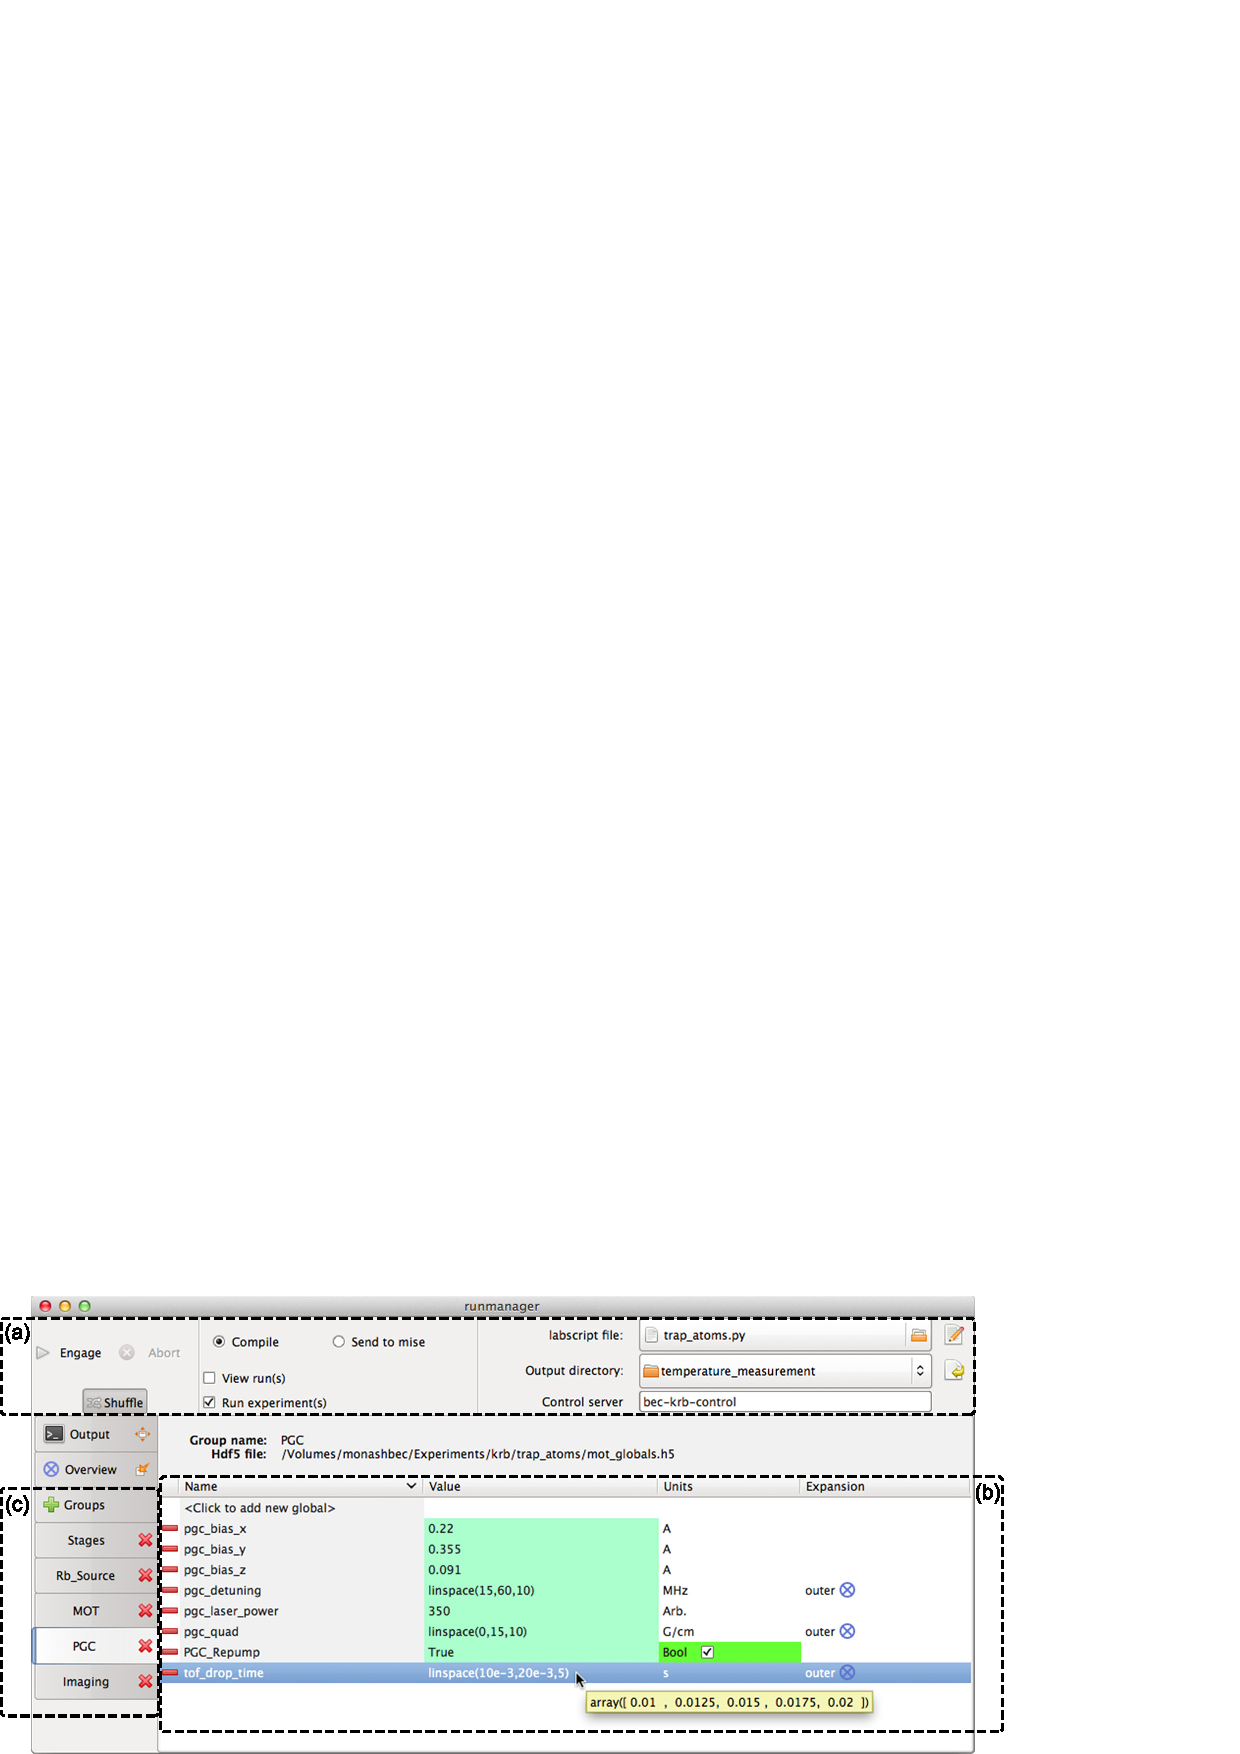
\includegraphics[width=\textwidth]{figures/software/new_screenshots/runmanager.png}
\caption{Runmanager as of 2018, showing the interface for entering `globals', so called because they appear to the user's code as global variables. Boolean globals can be turned on and off with a checkbox, and expressions resulting in an error are highlighted in red. The `expansion' column is how one chooses whether a global should be considered a list of values to loop over, re-running the experiment each time, and if so if that loop should be combined with other such globals to loop over the resulting product space (`outer') or whether the globals should be looped over together (`zip'). Zipped globals can be grouped together by typing a name in the expansion column to identify which `zip group' the global belongs to. Globals in the same zip group will loop together, and multiple zip groups will form separate axes of a product space.}\label{fig:runmanager}
\end{center}
\end{figure}

\subsection{runviewer}

[TODO SCREENSHOT]

Runviewer is a program for viewing the results of \texttt{labscript} compilation in the form of graphical plots of the voltages, digital values, frequencies etc that comprise the hardware instructions produced. This is useful for debugging experiment design and timing of instructions, as well as verifying that a newly made \texttt{labscript} device class (the `driver' code for each device that converts \texttt{labscript}'s intermediate description of hardware instructions into the actual format required for a given device) is functioning as intended.
\subsection{BLACS}

\begin{figure}
\begin{center}
\includegraphics[width=\textwidth]{figures/software/new_screenshots/blacs.png}
\caption{BLACS as of 2018}\label{fig:blacs}
\end{center}
\end{figure}

BLACS (Better Lab Apparatus Control System) is a graphical program responsible for queueing experiment shots as compiled by labscript and runmanager, and executing them one after the other on the hardware. As such, BLACS interacts with a number of python classes that function as \emph{drivers} for each devices, containing code that uses the required software libraries, hardware drivers or communication protocols to communicate with the devices in the manner required by each one individually. BLACS executes the code for communicating with each device in a separate process in order to isolate them from each other, so that communication failures, software bugs or other failures that may occur in the interactions with one device will not stop BLACS from continuing to function in other respects. Errors are presented graphically and each device process may be restarted with the click of a button if something goes wrong. This is useful for both responding to unexpected failure, as well as for debugging during the development of the driver for a new device (or of new features for an existing device) being integrated with the labscript suite.

Upon receiving an HDF5 file from \texttt{runmanager}, BLACS adds it to the queue of shots to be executed on the hardware. It then executes these shots in order, by programming the instructions stored in the HDF5 file into each device, and then giving the top level device the command to begin the experiment. Devices are programmed in parallel in their separate processes, saving time.\footnote{Particularly since many delays in programming the devices are communication delays, during which the process is simply idle.} Once the shot is complete, each device process is given the command to write any data acquired to the HDF5 file.

BLACS can also repeat shots, by copying and then `cleaning' an HDF5 file after it has already run to produce a new shot file ready to be run on the hardware. It can repeat either all the shots, or just the last one in the queue. This ability to always keep running by repeating the last shot in the queue is crucial for experiments using alkali metal dispensers (`getters') or desorbing metal vapour using UV desorption [CITE, check correct name], as these must run on an approximately fixed duty cycle to maintain the desired atomic vapour pressure. If the experiment stops running, it will have to `warm up' again.

\subsection{lyse}
\begin{figure}
\begin{center}
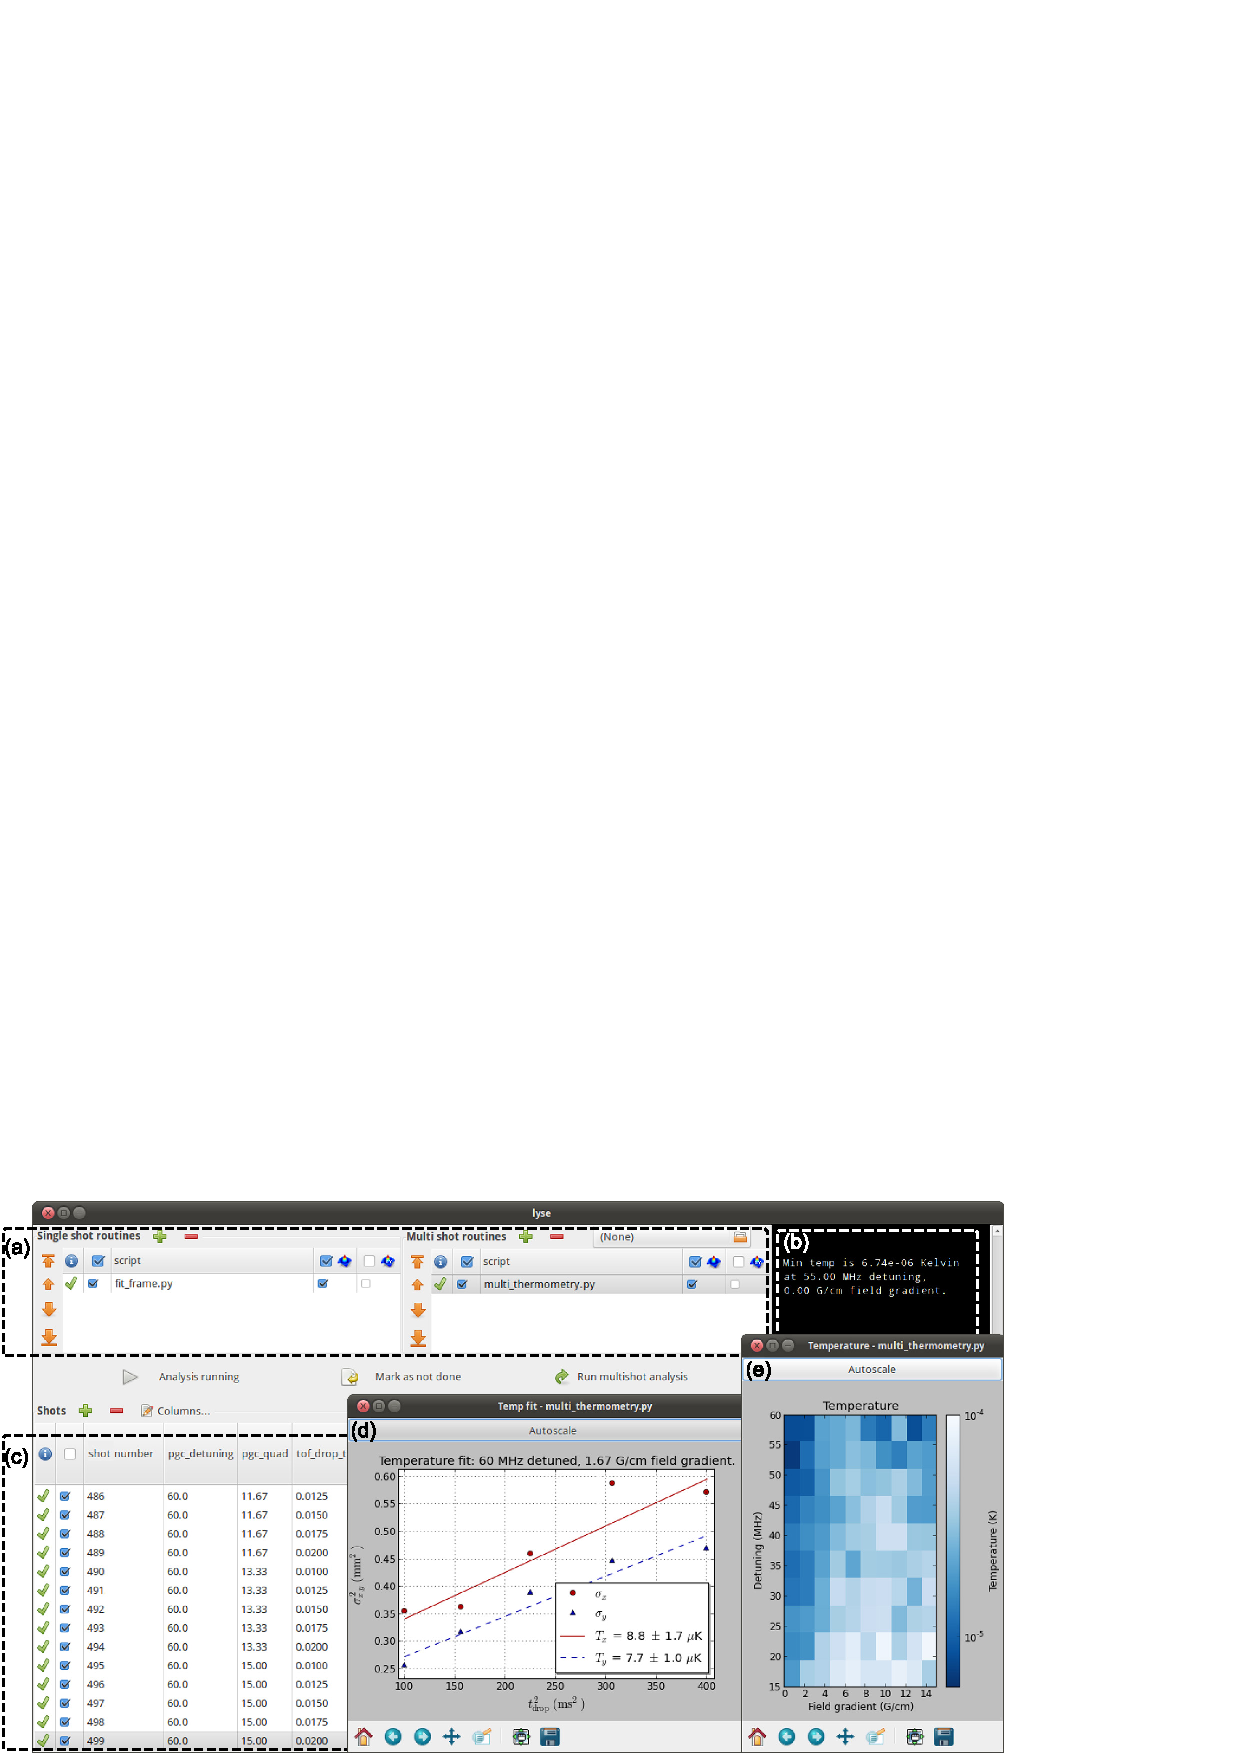
\includegraphics[width=\textwidth]{figures/software/new_screenshots/lyse.png}
\caption{Lyse as of 2018}\label{fig:lyse}
\end{center}
\end{figure}

Once BLACS is done with the experiment, the shot files are optionally passed on to the analysis program \texttt{lyse}. \texttt{lyse} is essentially a scheduler for user-provided analysis routines. A list of analysis routines (in the form of Python scripts), called \emph{single-shot routines} are executed in order whenever a new shot is received by \texttt{lyse}, with the shot file as input. The analysis routines may read raw data from the HDF5 file, or read analysis results saved by previously-run analysis routines, and save their own results. Analyis routines may also produce plots using the \texttt{matplotlib} library---\texttt{lyse} detects these and re-uses the same window for subsequent plots so that repeated runs of the analysis routines result in the plot updating in-place, rather than a proliferation of plot windows. Any other plotting library can be used (for example \texttt{pyqtgraph} [CITE]), though the user needs to write their code for the updating behaviour in this case.

The shot globals and analysis results for all shots received by \texttt{lyse} are maintained in a tabular data structure: a `dataframe' provided by the \texttt{pandas} [CITE] Python package, which is browsable in the \texttt{lyse} interface. This table of data is available to a further list of analysis routines, called \texttt{multi-shot\ routines}. This list of analysis routines is also run in sequence, but only once single-shot analysis has completed on all shots presently loaded into \texttt{lyse}. These routines can be analyses of relations between input parameters and analysis results of the shots, in order to say, measure a trend of the number of atoms in a MOT as the magnetic field gradient was varied. Both single-shot and multi-shot routines can be run from within lyse, or externally by running Python manually. In this latter case, the shot file on which to run single shot analysis can be provided as a command line argument, and the dataframe analysed by multi-shot routines will be obtained from a running instance of lyse over the network. This is no different to what happens when multi-shot routines are run from within lyse: they are simply run by lyse with no input, and are expected to call a function \texttt{lyse.data()} to obtain the dataframe. Because of the way this is implemented, one can also open an interactive Python interpreter on any computer on the same network, type \texttt{import lyse; df = lyse.data(hostname)} (where \texttt{hostname} is the hostname of the computer running lyse) and begin interactively exploring the data using the pandas library, one of its great strengths.

\section{Design philosophy and advantages of approach}

\subsection{It's code}
The design of our software brings the process of experimental physics closer to that of software development, making it amenable to many of the tools and processes in use in software development such as version control, bug tracking, textual diffs of what has changed in experiments. Both the experiment logic and the analysis routines comprise Python code that can be examined for changes using standard `diff' tools, stored in version control, or forked into multiple versions using distributed version control and merged back together again. This can allow risky changes to experiment logic or analysis code with the reassurance of being able to roll back to a known working state should the changes not prove fruitful. One exception to this `everything is code' philosophy is the globals themselves, they are stored in HDF5 files, though we do have a tool for `diffing' them too to highlight what has changed between two globals files, or between the current set of values configured in \texttt{runmanager} as compared to a particular shot file (\figref{fig:globals_diff}).

\begin{figure}
\begin{center}
\includegraphics[width=0.5\textwidth]{figures/software/globals_diff.png}
\caption{Helpful advice from a PhD student of the Spinor BEC lab}\label{fig:globals_diff}
\end{center}
\end{figure}

As in software development, experimental physics re-uses the same procedures time and time again, and needs a way to manage the complexity of turning large parts of functionality on and off. In a traditional atomic physics control system, disabling a part of the experiment logic might involve tedious clicking to remove or disable each instruction involved. In Python, this can be a single \texttt{if} statement wrapping a function call containing all the complexity of the part of the experiment being disabled. The ability of high level programming languages to manage complexity via encapsulation and code re-use with functions, classes and modules carries well over to experimental physics. Using an existing programming language saves us, as the developers of a control system from having to re-invent (likely badly) the features of a programming language within our control system. For example, the tedious clicking required to `comment out' part of an experiment in the aforementioned hypothetical `traditional' control system could be avoided if the system implemented a feature for this in particular. But then what about \emph{nested} if statements? To support all the use cases that might come up, one would have to essentially invent a programming language within such a control system. Instead of this, why not use an existing programming language?

The use of an existing programming language only aids the labscript suite in the case of `compile-time' conditionals and other control statements--- that can be evaluated when the hardware instructions are produced by labscript, as opposed to `run-time' when the experiment is run on the hardware (such as conditionally turning a laser on if a photon is detected on a photo-detector). These `run time' control statements do require special treatment in labscript, and labscript currently only has one type of functionality like this built-in. This is the ability to pause the experiment until a pulse is produced that resumes the master pseudoclock. This allows the common use case of synchronisation with the background $50\unit{Hz}$ magnetic noise from mains electricity by pausing the experiment until a fixed point in the $50\unit{Hz}$ cycle to ensure the magnetic field is close to identical from one shot to the next. It also allows servoing of the MOT load, by loading for a variable amount of time based on a threshold fluorescence such that variations in MOT loading efficiency from one shot to the next do not result in variations in actual atom numbers.

Further `run-time' control flow tools such as conditional branches would not be too difficult to incorporate into labscript in the future, but would require hardware capable of holding multiple alternative sets of instructions in memory and able to switch between them on receipt of a digital pulse on some input. The SpinCore PulseBlaster [R?]---the device used by most users of the labscript suite to produce clocking pulses---supports this [VERIFY], but most output devices labs use with the labscript suite do not.

\subsection{Coupled components and the Unix philosophy}

An aspect of the Unix philosophy [CITE] is that tools should `do one thing and do it well'. The components of the labscript suite are not as minimal as they could be, but are nonetheless separate components that talk to each other over network connections.\footnote{This is in violation of another part of the Unix philosophy that says programs should exchange text streams: our programs mostly exchange messages over network sockets, containing filenames pointing to HDF5 files on a network drive.} Thus in principle once can remove a component and replace it with another that plays a different role. For example, \texttt{runmanager} has been re-purposed by Philip Starkey [thesis in preparation] to generate parameter space scans for numerical simulations instead of experiments, by calling code other than labscript code. \texttt{lyse} is in use by one group [CITE THE GROUP? FRED] for on-line analysis of experiment results in the form of HDF5 files that were produced by Matlab code.

The separate programs of the labscript suite are also implemented in many cases as separate processes exchanging instructions over network sockets. Whilst these processes are so far running on the same computer, it is possible to extend them to run on separate computers merely by changing the hostname that the network sockets connect to from \texttt{'localhost'} to the hostname of some other computer (actually starting the other process on the other computer automatically whilst retaining security is another matter). This makes it not too large a modification to be able to have lyse analysis routines run on a remote computer (perhaps a server with a powerful GPU or many CPU cores for computationally intensive analyses), or to have devices controlled by \texttt{BLACS} be connected to a different computer than the one running \texttt{BLACS}. This latter configuration can aid in reducing the size of ground loops due to long cables, or allow the simultaneous use of devices that require different operating systems or other conflicting software or hardware configurations preventing them from being used on the same computer.\footnote{A pertinent example is the bandwidth of a computer's USB2 bus being the limiting factor in the speed at which one lab can run experiments: using two computers to program two USB devices could halve the programming time between shots}.

\texttt{runmanager} is a graphical program, but also a software library for setting globals and compiling shots by running labscript code, and so is in a sense two separate components. As a result, it is possible to write code that produces shots based on something other than the simple parameter space scans runmanager is capable of producing. In the past, the labscript suite contained a program called \texttt{mise}, used for performing optimisation of the experiment. \texttt{mise} would use the runmanager library (but not the graphical interface) to produce shots based on a genetic algorithm and the results of analysis communicated to it by \texttt{lyse} analysis routines. This type of optimisation was powerful, but has been superseded, and we no longer maintain \texttt{mise}. However a similar workflow is used in the spinor BEC laboratory at Monash to integrate the MLOOP machine-learning optimisation library with the labscript suite for experiment optimisation.

The separation of components also aids in development of the labscript suite. Programs can be ported to use updated versions of libraries one at a time, and tested separately, enabling a more flexible process of development.


\subsection{Off-the-shelf hardware}

The labscript suite is the software part of an experiment control system, and does not mandate any particular hardware. Whilst certain hardware drivers are developed and maintained by myself and the other labscript suite developers, if one wants to use different hardware, one can write drivers for it and use it with the labscript suite. This does mean that the software cannot make hard assumptions about the hardware and has to deal with a wider range of possibilities, which is a complicating factor in maintaining the code, but I believe this approach is the better one compared to having a limited range of hardware designed specifically for the labscript suite. It is hard to predict what hardware people will need for atomic physics experiments, and our efforts are better spent making software than hardware. Labscript developers and users have made some hardware of their own as well however, and there exists a low-cost pseudoclock and and a digital out device both based on a sub-\$100 microcontroller board [CITE SOMETHING? Phil, me, Martijn?]. However these have proved difficult to maintain in the face of changing software development kits for the microcontrollers, and I suspect FPGAs are a better solution. Rory Spiers [CITE thesis? Or say recently graduated Melbourne and now at JQI?] has developed a low-cost FPGA-based pseudoclock [not yet published] that may be an attractive alternative to the PulseBlaster.

\subsection{Open source Python}



open source and using open source libraries: advantage: patching upstream is a viable option. I have submitted and had patches accepted by numpy, pandas, h5py and pyzmq that improved their usability for specific use cases we have had. 

crowdsource bugfixes! Lots of competent programmers in physics groups. They implement long-standing features
that we have not had time to implement ourselves.

Popular, dynamic programming language
Allows us to hack on it to introduce custom behaviour whilst keeping the benefits of using a general purpose programming language. Allows new students to get up to speed quickly. Allows interoperability with a wide range of tools and protocols for talking to other code and to hardware.

Standard format: HDF5


\section{Recent developments}
Firstly, far more people using the software.

Since the paper:

General:
A port to the Qt GUI toolkit, which occured while I was in the US visiting Ian. This toolkit is more widely used and cross-platform.
A proper installer such that installation is now running one script and works reliably across platforms.
An (almost complete) port to Python 3
Mise is no longer used, instead people are plugging lyse and the runamnager API into things like MLOOP. This demonstrates the pluggability of the system, but could be improved.
General polishing all round
More devices
Output capturing of subprocesses now captures ouput of subsequent subprocesses and extension code
More flexible camera interfaces, there are several Python camera servers. We no longer treat cameras as special, and if they need to be on a different computer for reasons of hardware or screen real estate, the remote devices feature will get that.
A port to the Qt GUI toolkit

Delete shots functionality - lyse can deal with it and BLACS has a plugin to do it

Labscript:
Arbitrary function ramps
Markers
Inverted DO
Gated clocks: allow more devices to run off the same clock given very different memory capacities.

lkyse: copy to clipboard

BLACS:
Repeat functionality repeat last
Delete repeated shots
Plugin mechanism
Optional Terminals visible for all devices for debugging purposes
Can be started without a Connection table
Bugfixes leading to faster times in between shots

runmanager:
Saving and loading of configuration settings
Finer control over parameter spaces: per-axis shuffle, control over axis loop order
Agnostic compilation: can be used to make parameter space scans for arbitrary things

runviewer:
Saving and loading of configuration settings
nonlinear time (using markers)
dont' revernse engineer data? Save extra data? Maybe, maybe not.

lyse:
Copy figures to clipboard
Saving and loading of configuration settings
Can work with deleted shots
Performance ehancements

devices:
Supporing more devices and more modes of operation
Generic NI DAQmx
More PulseBLaster models
More modes of operation for the Novatech

\section{Future developments}

Analog input widgets for BLACS

Plugin tabs

Remote control of runmanager - makes it easier to implement optimisers and other feedback

Compile queue: just-in-time compilation so that feedback can be on a per-shot basis, so that repeated shots can take into account updated variables immediately

Integrate remaining features from another fork (spielman fork): postprocessing scripts for per-shot feedback, fixed-duration shots.

labscript rewrite for more precise and nondesctructuve control of timing

remote processes so devices can be connected to different computers

Progress bar in BLACS (can be coloured by markers)

Analysis globals

\section{Regrets, Antiregrets, and friction}
GTK. Bad call
Labscript processing should be integer based and nondestructive. Bad call, yet to fix

Friction:
pandas

Antiregrets
ZMQ and the zprocess module
Qt
Python 2
threading like crazy

\section{Reproduced publication: A scripted control system for autonomous hardware-timed experiments}
\includepdf[pages=2-]{labscript_paper/labscript_paper.pdf}


\setcounter{chapter}{4}

\chapter{Particle velocimetry of vortices in Bose–Einstein condensates}\label{chap:velocimetry}

\lettrine[lines=3]{T}{his chapter investigates}, via numerical simulation, an imaging method for the real time tracking of quantum vortices in a turbulent $^{41}$K condensate. The method involves ultracold $^{87}$Rb tracer particles that become bound to vortex lines in the condensate and are imaged continuously to track the vortex lines as they move. The imaging of tracer particles to track vortex motion has previously proved successful in superfluid helium~\cite{bewley_generation_2009, bewley_superfluid_2006, packard_vortex_1982}, and the method of laser cooling and imaging atoms in high resolution with the same laser light has also been successful in cold atom systems~\cite{bakr_quantum_2009}. This chapter presents the results of numerical simulations of the method under a number of assumptions to establish its feasibility as an imaging method. 

\begin{figure}
\begin{center}
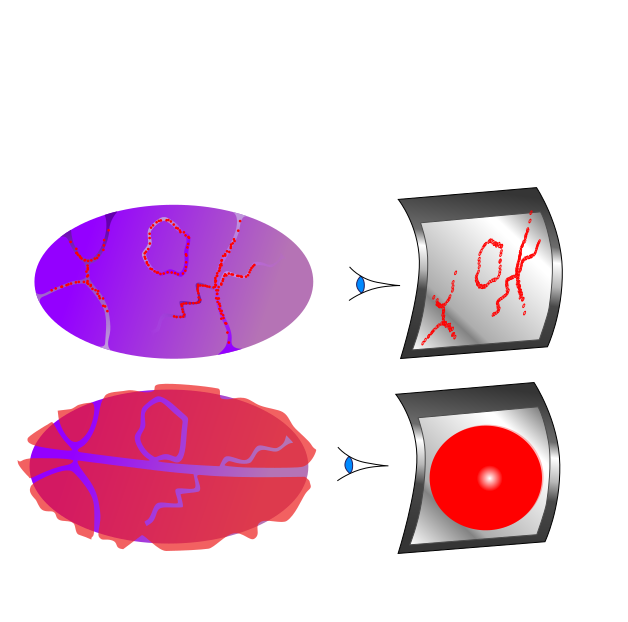
\includegraphics[width=0.6\textwidth]{figures/unsorted/side-on.pdf}
\caption{\label{fig:side-on}Imaging of the condensate itself, whether by flourescence (bottom) or absorption imaging makes it difficult to resolve vortices unless they are viewed end-on. The vortex cores are usually smaller than the imaging light's wavelength, and are thus also difficult to resolve unless the cloud is allowed to expand. Imaging tracer particles instead (top) has the potential to resolve both these problems.}\label{fig:side_on}
\end{center}
\end{figure}

This method has the potential to overcome several existing difficulties that typical imaging techniques face when used to image vortices. In ordinary absorption imaging, atoms are imaged via resonant absorption of the condensate itself, and vortices---visible as density minima---generally can only be seen when the vortex line is normal to the image plane. If not viewed end-on in this way, a vortex line represents only a minor decrease in column density and cannot be distinguished from the rest of the condensate (\figref{fig:side_on}). One solution to this problem is to slice the condensate into layers, and image them separately~\cite{anderson_watching_2001}.

The use of tracer particles that are only present within vortex cores allows vortex lines to be visible from any viewing angle.  Furthermore, since the atoms being imaged reside in the vortex cores themselves rather than the bulk of the condensate, this imaging can potentially be repeatedly or continuously performed without destroying the condensate. This may enable observation of the time evolution of Kelvin waves~\cite{bretin_quadrupole_2003}, vortex reconnections~\cite{leadbeater_sound_2001}, and vortex rings~\cite{anderson_watching_2001}.

This \emph{in-situ} imaging of vortex dynamics may allow more types of vortex motion to be imaged. Dynamics of \bec s are typically studied using a shot-by-shot method, in which repeated experiments with identical initial conditions are imaged destructively after being allowed to evolve for different amounts of time. Whilst this works for many types of dynamics, it fails for experiments that are sensitive to initial conditions and noise (quantum or otherwise), such as turbulent flow. This includes phenomena which cannot be created reliably in the same initial state, even though the evolution thereafter would be consistent from one experimental run to the next. One such phenomenon is the spontaneous generation of vortices after evaporative cooling~\cite{weiler_spontaneous_2008}.

\emph{In-situ} imaging of vortex motion has been achieved previously~\cite{freilich_real-time_2010}, by ejecting a fraction of the atoms from the condensate periodically and imaging them. This process is limited by depletion of the condensate, and was also used only to image vortices end-on. The fraction of the condensate being imaged was also allowed to freely expand before being imaged, since vortex cores are otherwise unable to be resolved by the wavelength of light used. Our proposed method would require neither free expansion or depletion of the condensate.

\section{Motivation: Turbulence}

It is commonly said that turbulence is one of the greatest unsolved problems of classical physics. But in what sense is it an unsolved problem? It is not a problem at all if your aim is reductionism---the Navier--Stokes equation adequately describes the evolution of a Newtonian fluid within its domain of validity, and the process of deriving it from the underlying motion of classical particles is well understood. It's turtles all the way down~\cite[p 1]{hawking_brief_1988}; what more could we ask for?

A demonstrative comparison might be with the field of thermodynamics, as precisely the same statement can be made about the energy content and exchange between systems of particles. Thermodynamics has revealed that despite the chaotic motion of individual particles in an ensemble, definite statements can still be made about the behaviour of the system as a whole, \emph{without having to consider the dynamics of the constituent components in detail}.

This is the kind of solution people have in mind when they speak of `solving' the problem of turbulence. Laws describing the average properties of a fluid without reference to its precise flow field would not simply be interesting as describing turbulence as an emergent phenomenon, but would aid practical computations, which for many problems of interest are prohibitively computationally expensive. The flow of a turbulent fluid contains detail on such a  wide range of length scales that finite-element or finite-difference analyses of a system such as an aeroplane wing requires a very high resolution in order to be accurate. Following an estimate of computing power required to simulate a turbulent system down to its smallest length scales, Stanley Corrsin quipped~\cite{corrsin_turbulent_1961}:
\begin{quote}
The foregoing estimate  is enough to suggest the use of analog instead of digital  computation; in particular, how about an analog consisting of a tank of water?
\end{quote}
The reliance of the aerospace industry on wind tunnels and practical tests shows that there is some truth to the necessity of using nature as one's computer when it comes to turbulence. Whilst nature must always have the final say, it would be of great benefit to be able to compute expected results more cheaply before setting up a wind-tunnel experiment or constructing a prototype aircraft.

But are we asking for too much? Perhaps the statistical properties of a turbulent fluid fundamentally cannot be decoupled from the finer details. There is reason to believe that this is not the case. There are several tantalising results that hint at universal properties that all turbulent flows share, and there is the simple empirical observation that the average flow of turbulent fluids at large scales is reproducible from one experimental run to the next~\cite[pp 13, 86]{davidson_turbulence:_2004}.

One of these universal results is Kolmogorov's theory of the statistics of small eddies~\cite{kolmogorov_local_1941, spalding_kolmogorovs_1991}. Another is the fact that the rate of energy dissipation via the action of viscosity at small scales is independent of the viscosity itself~\cite[p 77]{davidson_turbulence:_2004}.

Then there is the Richardson energy cascade~\cite{richardson_weather_2007}, in which energy is continually transferred from larger scales to smaller scales. With dissipation at the smallest scales and addition at larger scales, this allows for the existence of `steady state' turbulence.

The above examples derive from ordinary, viscous fluids. Bose--Einstein condensates on the other hand are superfluids. There are several interesting aspects of superfluid turbulence that differ from classical turbulence. The defining difference is the absence of viscosity; another major difference is the quantisation of circulation. On length scales much larger than spacing between vortex lines, superfluid turbulence is expected to closely resemble classical turbulence~\cite{tsubota_energy_2009}. At smaller scales however the energy dissipation mechanism is different, instead involving the production of sound waves via vortex interactions~\cite{tsubota_energy_2009, vinen_how_2005}.

In certain 2\textsc{d} geometries, an \emph{inverse cascade}~\cite{onsager_statistical_1949, kraichnan_inertial_1967} is predicted to take place in superfluids, whereby energy moves not from large scales to small, but from small to large, clustering quantised vortices of the same circulation direction together. This phenomenon has been studied theoretically and numerically in the Monash Quantum Fluids group~\cite{simula_emergence_2014, groszek_vortex_2018} and recently experimentally observed in the Monash Dual-Species laboratory in experiments performed by Shaun Johnstone~\cite{johnstone_order_2018}, simultaneously with a group at the University of Queensland~\cite{gauthier_negative-temperature_2018}.

The following definition of turbulence, taken from~\cite[p 53]{davidson_turbulence:_2004}, emphasises the role of vortices in turbulence in general:
\begin{quote}
Incompressible hydrodynamic turbulence is a spatially complex distribution of vorticity which advects itself in a chaotic manner in accordance with [the vorticity equation\footnote{Which is a transformation of the Navier--Stokes equation for an incompressible fluid into a form in which the vorticity field is center-stage.}]. The vorticity field is random in both space and time, and exhibits a wide and continuous distribution of length and time scales.
\end{quote}

When vorticity exists only in infinitely narrow lines, as it does in superfluid, the vorticity equation mentioned in the above definition reduces to a Biot--Savart type law which can be used to compute the motion of vortices without having to compute the entire flow field.

This is why we are interested in the study of the dynamics of quantised vortices. Unlike in classical fluids, the vortices in superfluids have a definite position and size; there is either a vortex at a given spatial location or there is not. This may make it simpler to describe the motion of vortices statistically.

So far experimental studies of superfluid turbulence have been primarily in the context of liquid helium~\cite{leggett_superfluidity_1999}. Bose--Einstein condensates offer a compelling alternative subject of study for superfluid turbulence. The high degree of control afforded over systems of cold atoms allows the superfluid's properties to be tweaked in several ways, creating a larger parameter space in which to study turbulence than that afforded by liquid helium.

\section{Overview of velocimetry scheme}

\begin{figure}
\begin{center}
\includegraphics[width=0.6\textwidth]{figures/unsorted/setup.png}
\caption{\label{fig:setup}The simplest scheme for cooling and imaging the tracer particles with the same light is polarisation gradient cooling, involving six slightly off resonant beams (red), with each counterpropagating pair having opposite linear polarisations. This will scatter some light off the tracer atoms, as well as cool them to sub-Doppler temperatures. If the cooling is sufficient, it should encourage the atoms into the vortex cores where their energy is lower, if they aren't already there. Both the rubidium tracers and the potassium \bec\ will be trapped with approximately the same trapping potential by a strong, far off-resonant laser (orange), via the dipole force. Magnetic trapping cannot be used, as polarisation gradient cooling does not work in the presence of a magnetic field.}
\end{center}
\end{figure}

As mentioned, the core idea of our proposed imaging method is to use tracer particles to track vortex cores in a \bec\ in real time. In this chapter I consider $^{87}$Rb atoms as tracer particles in a \textsc{bec} made of $^{41}$K. This choice is due to the strong interspecies repulsion between these atomic species, which gives rise to the trapping of atoms in the vortex cores. In the limit of low densities and temperatures, such that three body collisions are suppressed and $s$-wave scattering dominates the interspecies interactions~\cite[p 120]{leggett_quantum_2006}, the rubidium tracer atoms experience a potential due to the potassium:

\begin{equation}
V(\vec{r}) = \frac{2\pi\hbar^2 a_s}{m_r}\rho_\up{K}(\vec{r}),
\end{equation}
where $\rho_\up{K}(\vec{r})$ is the spatially varying atom density of the potassium condensate, $a_s$ is the interspecies $s$-wave scattering length, and
$m_r = \frac{m_\up{K}m_\up{Rb}}{m_\up{K} + m_\up{Rb}}$ is the reduced mass of the scattering pair. Vortex cores thus create potential wells for other atoms, since they are regions of low condensate density in a background of high density.

The basic setup of the scheme is shown in Figure~\ref{fig:setup}. Cold rubidium atoms are introduced (such as by magnetic transport from a \mot) to a potassium condensate, after which both species are optically trapped at the focus of a high power $1064$nm laser, using the dipole force. Various methods may be used to create vortices in the condensate. These include bluff-body flow, where a repulsive potential is dragged through the condensate, and inducing a turbulent state by applying off-resonant laser speckle. The rubidium atoms are then expected to become trapped in the low density vortex cores.

The atoms are imaged with resonant or near-resonant laser light, depending on the exact scheme employed. In this chapter I present the results of simulating two configurations, one of which has near-resonant laser light also cooling the atoms to keep them trapped in the vortex cores, and the other relying solely on sympathetic cooling with imaging being performed with resonant light.

The simplest scheme which attempts to cool the rubidium atoms is ordinary polarisation gradient cooling, in which the same light is used for imaging and cooling the atoms (Figure~\ref{fig:setup}). This was considered in my Honours thesis~\cite{billington_particle_2010}, the results of which I summarise in the next section. This method precludes the use of a magnetic trap or large bias field, since either would destroy the cooling effect.

The vortex potentials may be made deeper through the use of a Feshbach resonance (Section~\ref{sec:feshbach}), which increases the interspecies scattering length. However, since this requires a magnetic field, it precludes the use of ordinary polarisation gradient cooling. In section (see Section~\ref{sec:laser_cooling_simulations}) I present an alternative polarisation gradient cooling scheme designed work in the presence of a magnetic field of the strength required for the Feshbach resonance of interest.

Effective imaging of vortex motion would require approximately $10^5$ photons per second to scatter off each rubidium atom without it escaping its vortex core trap, and without causing so much heating as to destroy the condensate on a reasonable experimental timescale. A high resolution, low aberration lens (numerical aperture $\approx 0.5$) would also be required to focus the scattered light onto a fast capture, high quantum efficiency camera to produce images of vortex motion.

\section{Relation to previous work}

This scheme was first investigated in my Honours project~\cite{billington_particle_2010}. In that work I investigated the ability of vortex potentials to trap atoms, including consideration of the depth of such traps when measured in units of the photon recoil energy. Considering the depth in these units was a first attempt to estimate how easily atoms may escape vortex potentials in the presence of imaging light. Figure~\ref{fig:levels1e14} and Figure~\ref{fig:levels1e15}show bound states of typical vortex potentials at different condensate densities.

\begin{figure}
\centering
\noindent\makebox[\textwidth]{
\includegraphics[width=0.5\columnwidth]{figures/velocimetry/levels1e14_l=00.png}
\includegraphics[width=0.5\columnwidth]{figures/velocimetry/levels1e14_l=01.png}}
\noindent\makebox[\textwidth]{
\includegraphics[width=0.5\columnwidth]{figures/velocimetry/levels1e14_l=02.png}
\includegraphics[width=0.5\columnwidth]{figures/velocimetry/levels1e14.png}}
\caption{Energy eigenstates of a rubidium atom in a potassium vortex core, for a potassium \textsc{bec} with background density $\approx 10^{14}\unit{cm}^{-3}$. There are a number of bound states spanning three orbital quantum numbers. Plots of the bound states are of a cross section through the centre of a vortex core, and the lower right plot shows just the energy levels. Figure reproduced from~\cite{billington_particle_2010}.}%
\label{fig:levels1e14}%
\end{figure}

\begin{figure}
\centering
\noindent\makebox[\textwidth]{
\includegraphics[width=0.5\columnwidth]{figures/velocimetry/levels1e15_l=00.png}
\includegraphics[width=0.5\columnwidth]{figures/velocimetry/levels1e15_l=01.png}}
\noindent\makebox[\textwidth]{
\includegraphics[width=0.5\columnwidth]{figures/velocimetry/levels1e15_l=02.png}
\includegraphics[width=0.5\columnwidth]{figures/velocimetry/levels1e15_l=03.png}}
\noindent\makebox[\textwidth]{
\includegraphics[width=0.5\columnwidth]{figures/velocimetry/levels1e15_l=04.png}
\includegraphics[width=0.5\columnwidth]{figures/velocimetry/levels1e15_l=05}}
\noindent\makebox[\textwidth]{
\includegraphics[width=0.5\columnwidth]{figures/velocimetry/levels1e15.png}}
\caption{As in Figure~\ref{fig:levels1e14}, but for a potassium \textsc{bec} with background density ${\approx 10^{15}\unit{cm}^{-3}}$. There are bound states over six different orbital quantum numbers. This vortex potential is much deeper than that in Figure~\ref{fig:levels1e14}, showing the effect of condensate density on the depth of the vortex potentials. Figure reproduced from~\cite{billington_particle_2010}.}%
\label{fig:levels1e15}%
\end{figure}

There were a number of conclusions from this investigation. Firstly, to minimise the recoil energy, rubidium is a better choice for tracer particle than potassium due to its larger mass, enabling a rubidium atom to remain trapped after scattering a number of photons that would cause a potassium atom to escape the same potential. Secondly, vortex potentials are not very deep when measured in recoil energies, and their depth depends strongly on the density of the \textsc{bec}. At typical condensate densities of $10^{14}\unit{cm}^{-3}$, the vortex potentials are expected to only be one or two recoil energies deep, making it unlikely that atoms could scatter many photons whilst remaining trapped in them. At larger densities of $10^{15}\unit{cm}^{-3}$, the vortex potentials are closer to $20$ recoil energies deep, making imaging of trapped tracer atoms more plausible.

The main simulation result of my Honours project considered a potassium condensate with a peak density of $10^{15}\unit{cm}^{-3}$ and rubidium tracer atoms being cooled using standard polarisation gradient cooling with parameters chosen to ensure each atom scattered $10^5$ photons per second in two spatial dimensions. The result was that initially randomly distributed rubidium atoms were able to become and remain trapped in the vortex cores whilst being cooled (Figure~\ref{fig:hybrid}).

\begin{figure}
\centering
\noindent\makebox[\textwidth]{\includegraphics[width=1.0\columnwidth]{figures/velocimetry/hybrid1.png}}
\noindent\makebox[\textwidth]{\includegraphics[width=1.0\columnwidth]{figures/velocimetry/hybrid2.png}}
\noindent\makebox[\textwidth]{\includegraphics[width=1.0\columnwidth]{figures/velocimetry/hybrid3.png}}
\caption{The result from~\cite{billington_particle_2010} of a two-dimensional hybrid quantum-classical simulation for 1000 classical rubidium atoms (right, depicted as fluorescence assuming diffraction through an $\mathrm{NA}=0.5$ imaging system) and a turbulent potassium \textsc{bec} (left) of peak density $\approx 10^{15}\unit{cm}^{-3}$. The rubidium atoms are subject to a classical approximation of the force due to polarisation gradient cooling as described in~\cite{billington_particle_2010}. Most rubidium atoms eventually either become bound to a vortex core or leave the condensate. Figure reproduced from~\cite{billington_particle_2010}.}%
\label{fig:hybrid}%
\end{figure}

However, the density assumed in this simulation was rather high for a real experiment. Three-body losses tend to limit the lifetime of condensates at such a high density, and so the work in this chapter investigates ways to make particle velocimetry work in a less dense condensate. As the vortex potentials are so shallow at lower density, as mentioned earlier the potentials may be deepened through the use of a Feshbach resonance.

In Section~\ref{sec:sympathetic} I consider a similar configuration, but with a more reasonable \textsc{bec} density combined with an enhancement of the interspecies repulsion due to a Feshbach resonance. I investigate whether sympathetic cooling of the tracer atoms by the condensate may be enough to keep them trapped in the presence of imaging light. Then, in Section~\ref{sec:laser_cooling_simulations} I present simulation results of a new laser cooling scheme designed to work at the magnetic field strength required for the Feshbach resonance.

\section{Sympathetic cooling}\label{sec:sympathetic}

The simulation performed in my Honours thesis considered only polarisation gradient cooling counteracting the heating effect of the imaging light. In reality, collisions between tracer atoms and atoms in the condensate would also contribute to cooling. This sympathetic cooling of the tracer atoms---which would also lead to heating of the condensate---was disregarded in my Honours thesis' results. 

Depending on the strength of the cooling effect from sympathetic cooling, this cooling may be sufficient to retain tracer atoms in vortex cores in the absence of an additional cooling mechanism such as polarisation gradient cooling. If laser cooling is not necessary to trap tracer atoms in vortices, then the Feshbach resonance may be used to enhance the interspecies scattering length, further enhancing the ability of the vortices to trap tracer atoms. In this section I consider a similar simulation to that in my Honours thesis, in which the tracer atoms are subject to sympathetic cooling only, in order to examine this possibility.

\subsection{Model}

As with the simulation in my Honours thesis, in this section I model the tracer particles classically in a \textsc{bec}

In this section I model sympathetic cooling due to elastic two-body scattering between the rubidium tracer atoms and the potassium atoms in the condensate. The model is two-dimensional, approximating a pancake-shaped condensate.

The potassium condensate is modelled with the Gross--Pitaevskii equation:

[BLAH]

where [define symbols], and the rubidium atoms follow the classical equation of motion

[blah]

where [define symbols].

The motion of the tracer atoms is punctuated by velocity jumps due to scattering of imaging photons and to two-body collisions with the condensate. The effect of photon scattering is modelled as velocity jumps of magnitude [RECOIL MOMENTUM EQUALS EXPRESSION] in a random direction projected into the 2D plane [VERIFY] of the simulation, occurring at random times at an average rate given by the photon scattering rate. The latter modelled as elastic collisions between a rubidium atom with the given classical velocity, and a potassium atom of velocity equal to the superfluid velocity [SYMBOL] of the condensate at the location of the tracer atom:

[EXPRESSION FOR SUPERFLUID VELOCITY]

The rate of two body collisions is given by the scattering cross section times the relative velocity or something like that:

[EXPRESSION]

Where the scattering cross section is - uh, check how I calculated it, it involves a Feshbach resonance obviously. At low temperatures $s$-wave scattering dominates so we're just using that.


\subsection{Results}

DEFINE EVERYTHING TURBULATE INITIAL CONDITIONS, REFER TO NUMERICS SECTIONS

\section{Sisyphus cooling in a $34\unit{G}$ magnetic field}\label{sec:laser_cooling_simulations}

As mentioned, one of the limitations of the usual method of polarisation gradient cooling is that it doesn't work in a magnetic field. Usually this is not an issue for the cooling stage used en-route to \bec; the magnetic field is simply temporarily switched off. Our imaging method would benefit from a cooling scheme that does work in a magnetic field, since the repulsive interactions between $^{87}$Rb and $^{41}$K can be greatly enhanced via a Feshbach resonance at $34 \unit{G}$~\cite{thalhammer_double_2008}. This would make the potential wells that the rubidium atoms see deeper, trapping them more strongly. However if the magnetic field destroys the cooling mechanism then the atoms won't stay trapped for long. Even if sympathetic cooling is sufficient to image tracer particles trapped in vortices, the addition of a cooling scheme would increase the lifetime of the condensate on account of decreased sympathetic heating, and may allow a larger scattering rate of photons before the tracer atoms cease to be trapped.

The Feshbach resonance only occurs if both species are in their respective \mbox{$|F=1,m_F=1\rangle$} spin state,\footnote{$F$ is not a good quantum number in a nonzero magnetic field, so what we mean writing this is the state that one would get if starting in an $F$ state and adiabatically turning on the magnetic field.} so a cooling mechanism in which the rubidium atoms spend a significant fraction of their time in this state is desirable.

In this section I present a sub-Doppler cooling scheme that is designed to cool $^{87}$Rb in a $34\,$G magnetic field. The basic Sisyphus mechanism---of atoms moving alternately between spin states which see different potentials---is possible to find in many multi-level systems of sufficient complexity\footnote{And indeed, many other Sisyphus cooling mechanisms exists other than polarisation gradient cooling~\cite[p 116]{metcalf_laser_1999}.}; my cooling scheme uses a Sisyphus mechanism with four lasers to cool and repump $^{87}$Rb atoms in a $34\unit{G}$ field, with the atoms spending approximately half their time in the \mbox{|$1,1\rangle$} state.

In Section~\ref{sec:vortexcooling}, I briefly describe another cooling scheme suggested by Kris Helmerson, which uses the vortex cores themselves as the potential hills in a Sisyphus mechanism. I have not simulated this scheme to asses its viability; I mention it here because it is illustrative of the type of problem that is difficult to model semiclassically, and was one of the factors that led me to consider the use of hidden variables in semiclassical models, as discussed in Chapter~\ref{chap:hvsc}.


\subsection{Description of cooling scheme}

\begin{figure}
\begin{center}
\includegraphics[width=0.65\textwidth]{figures/unsorted/cooling_simplified.pdf}
\caption{\label{fig:cooling_simplified}An idealised depiction of the cooling scheme, with repump lasers and undesired states not shown. Two lasers on the D$_1$ line are used for cooling, both linearly polarised, and arranged so as to form two interleaved standing waves. Both are blue detuned from the transitions they target, and they differ by about $6.8\,$GHz. This difference means that the alignment of the two standing waves can only be maintained over a distance of about a centimetre.}
\end{center}
\end{figure}

The scheme involves four lasers, two for cooling and two for repumping. For simplicity I will first focus on the cooling lasers only, depicted in Figure~\ref{fig:cooling_simplified}. Imagine that we have a rubidium atom at $z=0$ and in the $|1,1\rangle$ hyperfine groundstate. Here our atom sees no light, as the intensity of the cooling laser labeled $\omega_1$ is zero, and it is in the wrong state to be pumped by the $\omega_2$ laser (which is not resonant with any transitions from the $|1,1\rangle$ groundstate).

As our atom moves rightward however, it will have to climb the repulsive potential hill formed by the $\omega_1$ laser. As it does so, its $|1,1\rangle$ excited state probability will increase, and along with it, the probability of spontaneous emission. Spontaneous emission will be most likely to occur near the top of the potential hill where the laser intensity---and hence the excited state probability---is greatest.

The most likely groundstate for the atoms to decay to from the $|1,1\rangle$ excited state is the $|2,2\rangle$ groundstate, and this is most likely to occur near $z=\frac\lambda4$. If this occurs, we now have an atom in the $|2,2\rangle$ groundstate at $z=\frac\lambda4$, a situation similar to that in which it started. Again, out atom now sees no light, but which laser has zero intensity and which targets the wrong transition are swapped.

As our atom continues rightward, it now has to contend with the potential hill formed by the $\omega_2$ laser, and is most likely to undergo spontaneous emission from the $|2,2\rangle$ excited state near the top of the potential hill. This time emission is most likely to put the atom into the $|1,1\rangle$ groundstate.

This process repeats, with atoms repeatedly climbing potential hills and being cooled. They spend approximately half their time in the $|1,1\rangle$ groundstate, allowing us to take advantage of the strong interspecies repulsion that that state entails for our two atomic species.

Of course, as is always the case, things aren't that simple. Whilst the two spontaneous decays mentioned above are the most likely, they are by no means the only possibilities. Some spontaneous decays will put the atoms back into the groundstate from which they came, with no harm done except a little extra heating from the photon recoil. Other decays however will put our atom into states that are not involved in the cooling scheme, where they will remain with no further cooling unless we do something about it. For this we need repump lasers (Figure \ref{fig:cooling_full}).

There are three states that the atom might end up in as a result of decay from the two excited states involved in the cooling process, and two repump lasers are used to excite them to three $P_\frac32$ states. Two of these transitions are similar enough that they can be addressed with the same laser.

\begin{figure}
\begin{center}
\includegraphics[width=0.65\textwidth]{figures/unsorted/cooling_full.pdf}
\caption{\label{fig:cooling_full} The full cooling scheme, including repump lasers (yellow), cooling lasers (blue and green), and all possible decay paths (red). The repump beam which is drawn in between two ground and excited states has a frequency equal to the average of those two transitions. }
\end{center}
\end{figure}

\subsection{Methods}

This scheme was simulated for the case of a single atom, with the internal state of the atom modelled with the Schr\"odinger equation in the spin basis, the state vector being a complex 32-vector\footnote{One complex number for each state in \figref{fig:cooling_full}.}. The coupling terms between each pair of states were computed by solving the eigenvalue problem in the spin basis, with the Hamiltonian including Zeeman terms, and projecting the resulting eigenvectors onto the zero field eigenvectors. The zero field eigenvectors have known coupling constants\footnote{Using the dipole approximation and the rotating wave approximation, as described in Section~\ref{sec:optical_dipole_transitions}}, a weighted sum of which gives the coupling constants for the states at higher field\footnote{Each energy eigenstate at nonzero field is a superposition of exactly two of the zero-field eigenstates.}. Since the coupling constants are dependent on the laser intensity, they were re-computed constantly as the atom moved through different intensities of the cooling beams. This process produced a set of 32 coupled differential equations for the complex amplitudes of each state~\cite[p 4]{metcalf_laser_1999}, of the form :

\begin{equation}
i\hbar\frac{dc_e(t)}{dt} = -\frac12e\sum_{g,\ n} E_n \langle g |  q_n | e \rangle c_g(t) \ee^{-\ii\delta_{nge}t},
\end{equation}
and
\begin{equation}
i\hbar\frac{dc_g(t)}{dt} = -\frac12e\sum_{e,\ n} E_n \langle g |  q_n | e \rangle c_e(t) \ee^{\ii\delta_{nge}t},
\end{equation}
where each $c(t)$ is the complex amplitude of one state; the $e$ indices are over the excited states and the $g$ indices over the groundstates\footnote{not to be confused with the electron charge or base of the natural logarithm, also used but not as indices.}; the $n$ indices are over the lasers, with $E_n$ being the amplitude of the $n$\textsuperscript{th} laser's electric field, $\delta_{nge}$ the detuning of the $n$\textsuperscript{th} laser from the transition between the $g$\textsuperscript{th} ground and $e$\textsuperscript{th} excited states, and $\langle g |  q_n | e \rangle$ the dipole moment between the $g$\textsuperscript{th} ground and $e$\textsuperscript{th} excited states for the polarisation of the $n$\textsuperscript{th} laser.

The external motion of the atom was modelled classically, with the atom having a definite position and velocity in one dimension. The force on the atom was computed using the gradient of the light shift that the two groundstates experience due to the standing waves formed by the cooling beams \cite[eqn 3.16, p 33]{metcalf_laser_1999}. The atom's state was projected onto the two groundstates which see the cooling lasers. The resulting force on the atom was used in the classical equation of motion.

Spontaneous emission was handled by at each integration timestep, summing up all the population in $P_\frac12$ and $P_\frac32$ excited states, weighted by their decay rates (equal to the natural linewidth). This gave the probability of decay per unit time. Multiplying by the duration of one timestep, and comparing with a random number then determined whether a decay was to occur.

In the event of a decay, one excited state was randomly chosen, weighted by their populations, and then one groundstate, weighted by the transition strengths from the excited state. All population was then put into that groundstate and the simulation continued, with one photon's worth of momentum in a random direction added to the atom's external state to account for photon recoil.

The equations of motion were solved using fourth order Runge--Kutta integration, with the error monitored by verifying that the overall probability summed over all states remained close to unity.

\subsection{Results}

\begin{table}
    \renewcommand{\arraystretch}{2.0}
    \makebox[\textwidth][c]{
    \begin{tabular}{|c|p{3.5cm}|r|r|c|}\hline
    Type & Transition(s) targeted & Detuning & Intensity (per beam) & Polarisation\\\hline
    cooling (standing wave) & $|S_\frac12,2,2\rangle\rightarrow |P_\frac12,2,2\rangle$ & + $66.6\,$MHz & $5.0\,$mW$\,$cm$^{-2}$ & $\pi$ \\
    cooling (standing wave) & $|S_\frac12,1,1\rangle\rightarrow |P_\frac12,1,1\rangle$ & + $31.9\,$MHz & $5.0\,$mW$\,$cm$^{-2}$ & $\pi$ \\
    repump (single beam) & \parbox{5cm}{\ \\ $|S_\frac12,2,1\rangle\rightarrow |P_\frac32,2,2\rangle$ \\
                           $|S_\frac12,2,0\rangle\rightarrow |P_\frac32,2,1\rangle$} & Midway between & $50.0\,$mW$\,$cm$^{-2}$ & $\sigma^+$ \\
    repump (single beam) & $|S_\frac12,1,0\rangle\rightarrow |P_\frac32,1,1\rangle$  & $0$ & $10.0\,$mW$\,$cm$^{-2}$ & $\sigma^+$ \\

    \hline
    \end{tabular}
    }
    \caption{The parameters used in the laser cooling simulations. There are four lasers, each with a specified polarisation, intensity, and detuning from the transition it targets.}\label{table:numbers}
\end{table}

The laser parameters used in the simulation are shown in Table \ref{table:numbers}. The magnetic field strength used was 34$\,$G.

The simulation was run for 715 million integration timesteps of 20 picoseconds each\footnote{Which is about ten timesteps per oscillation of the fastest oscillating terms, which oscillate at a rate equal to approximately half the 6.8GHz hyperfine splitting of the rubidium groundstates.}, for a total of 14.3 milliseconds of simulation time. This took 14 days of computer time. In that time, the atom moved a maximum distance of 26 micrometres from its starting position, and its final position was 790 nanometres from its starting position. The atom's initial velocity was 195 millimetres per second, and during the simulation it reversed the direction of its velocity 2226 times. 4103 photons were emitted, for an average scattering rate of 2.87$\times$10$^\up{5}$ photons per second.

Computing the time averaged energy of the atom over the whole simulation using:
\begin{equation}
\langle E \rangle = \frac12 m_\up{Rb} \langle v^2 \rangle,
\end{equation}
and converting to temperature units with $k_B T = \langle E \rangle$ gives a temperature of $8.1\,\upmu$K. Since this is only a one-dimensional simulation, a temperature approximately three times higher would be expected in three dimensions, as the atom would have approximately the same amount of energy in each spatial degree of freedom.

A histogram of what fraction of the time the atom spent at different velocities is show in Figure \ref{fig:cold_atom}.

\begin{figure}
\begin{center}
\includegraphics[width=\textwidth]{figures/unsorted/cold_atom.pdf}
\caption{\label{fig:cold_atom} Histogram of atom velocity over time, normalised such that it can be interpreted as a probability density. A best-fit Maxwell-Boltzmann distribution is shown as the dotted line. It is no surprise that it is not a good fit---there is no thermalisation happening since we have only one atom and no collisions. The average energy is more informative than the fit parameters for determining the temperature that an ensemble of such atoms would have if they were allowed to thermalise. This is because the average energy would stay constant throughout thermalisation, whereas the fit parameters would not. Only for a fully thermal distribution would the two methods agree. The long tail visible to the right is the atom's initial slowdown from its starting velocity.}
\end{center}
\end{figure}

This one-dimensional temperature corresponds to approximately 44 recoil energies, and if extrapolated to three dimensions, about 132 recoils. Given that the potassium vortex potentials are at most about 15 recoils deep without a Feshbach resonance, and only about 8 recoils when you consider that the rubidium is not in the ideal state half of the time, this result will only be able to keep rubidium atoms trapped in vortex cores if we can get a factor of 20 or so increase in the interspecies repulsion via a Feshbach resonance.

This simulation has not, however, been optimised. Whilst some parameters were computed from others based on assumptions about optimal scattering rates and the like, no attempt has been made to scan over parameter space to see if the temperature can be made lower. I plan on using a genetic algorithm to optimise the parameters by managing a population of simulations running on one of the university clusters. A significant speed up should be possible by excluding from the simulation the atomic states that were shown in the first run never to become occupied. This will eliminate approximately two thirds of the states, and since the simulation is quadratic in the number of states, this should provide an approximately $10\times$ increase in simulation speed.

The simulation will also require repetition to verify that the results still hold when a significant error, recently discovered, is corrected. The error is that the Zeeman sublevels used in the simulation were all incorrect by a sign. There is a large degree of symmetry with this change, and the scattering rates between all involved states are almost identical, so I am confident that this will only slightly change the results.

Ultimately only experimentation will show whether this method is viable, and what the optimal parameters are, but since it requires a large number of lasers, it is likely worth further theoretical investigation before attempting to implement it.

\subsection{Vortex-assisted Sisyphus cooling}\label{sec:vortexcooling}

[COMMENT ON HIDDEN VARIABLES - PRESENTED HERE TO MAKE A POINT]

Another idea for a cooling scheme is to use the vortex potential itself as a spatial discriminator for transferring atoms between states. Similar to how a \mot\ traps atoms by bringing them into resonance with optical pumping only when they are some distance from the trap's centre, we could use the shape of the vortex potential to bring an \rf\ or microwave transition into resonance only when trapped tracer particles are some way up the side of a vortex core.

\begin{figure}
\begin{center}
\includegraphics[width=0.7\textwidth]{figures/unsorted/vortexcooling.pdf}
\caption{A basic description of the vortex-assisted cooling scheme.
\protect\\
1. The rubidium atom in its $|1,1\rangle$ groundstate repeatedly scatters photons from the laser marked with the blue arrow, climbing the vortex potential as it does so. The optical transition's linewidth is large enough that the energy shift due to the vortex potential does not move it off resonance.
\protect\\
 2. An \rf\ or microwave transition however, has an extremely narrow linewidth; its effective linewidth is dependent only on the \rf/microwave power. A microwave transition (grey arrow) comes into resonance only when the atom moves sufficiently far from the vortex core's centre, and coherently transfers population into the $|2,2\rangle$ groundstate.
 \protect\\
 3. The atom oscillates back and forth in the much shallower vortex potential that its $|2,2\rangle$ groundstate experiences. It is pumped weakly by the laser marked with the green arrow, and after a random time delay (and hence at a random position) spontaneously decays back to the $|1,1\rangle$ groundstate.
}\label{fig:vortexcooling}
\end{center}
\end{figure}

The basic idea is outlined in Figure~\ref{fig:vortexcooling}. In the presence of the Feshbach resonance, atoms in the $|1,1\rangle$ state will scatter some tens of photons, using whichever transition is most likely to have them decay to the same groundstate with minimal repumping (transitioning to the $|0,0\rangle$ excited state on the $D_2$ line looks to be the best choice). As the atom scatters photons, it climbs the side of the vortex potential, converting its new found kinetic energy (from photon recoil) into potential energy.

Due to the state-dependence of the interspecies scattering length, the vortex potentials for different states have different depths. This means that the \rf\ or microwave frequency required to transition between the different hyperfine states and Zeeman sublevels varies as a function of space, and can be tuned so as to only be resonant with atoms which have nearly escaped the vortex core.

The atom is then transferred into a different hyperfine or Zeeman state (the $|2,2\rangle$ groundstate should suit) and the hope is that it then lacks the kinetic energy to escape the (shallower) vortex potential it now finds itself in. Rather, it will oscillate back and forth in the well until a weak laser pumps it back into the $|1,1\rangle$ groundstate via spontaneous emission from some excited state (again chosen to maximise the decay probability to $|1,1\rangle$; the $|2,2\rangle$ $P_\frac32$ excited state looks to be a good choice.)

If this goes to plan, statistically the atom will be closer to the center of the  $|1,1\rangle$ vortex potential than when it left. Provided its corresponding drop in potential energy makes up for all the photon scattering (which provides fluorescence imaging), then we have a cooling scheme. It is yet another Sisyphus effect, with the atom climbing steep vortex potential hills and descending shallower ones.

This scheme will be simulated to determine its viability; preliminary calculations haven't turned up any problems yet.

% Paths: bilbo.tk: ~/laptop_backup/Desktop/current_work/sympathetic_cooling/
%                  ~/oldserver/bilbo/particle_tracking_higher_scattering_length
%                  ~/laptop_backup/Desktop/current_work/paper%20simulations/
%                  ~/laptop_backup/Desktop/current_work/paper
%                  ~/laptop_backup/Desktop/current_work/DPGPoster
% Compare to honours thesis - don't include stuff already in honours thesis!



\setcounter{chapter}{5}

\chapter{Hidden variables for semiclassical models with state-dependent forces}

Define/describe what a hidden variable theory is, drawing heavily on Aaronson's~\cite{Aaronson2005} explanations. Give examples, argue why the Schrodinger theory is appealing.

Motivate with Stern-Gerlach experiment, and derive the method, show what sorts of problems it
solves and where it disagrees with other models, provide simulation results. Limitations: no time dependent potentials, no 3D.

Possibly include speculation about these:

Maybe include a test to see whether it actually does work in 3D as-is, since we haven't actually checked, we just haven't been able to show on paper that current behavior is correct in 3D (also haven't shown it's incorrect).

Time dependent potentials could potentially be handled by approximating unitary as product of part due to spatial variation in H, and part due to time variation in H. compute transition probs for both such that a transition can be attributed to one or the other - only do velocity jumps to conserve potential if due to spatial motion, as time dependent potential can exchange energy with particle.

Matrix scaling for Schrodinger theory, discuss methods: Sinkhorn-Knopp, Lineal, and my one. Compare time complexity of algorithms so as to define the computational complexity of the hidden variables semiclassical method. Method is of course parallelisable on GPU or similar so is fast on parallel machines even if matrix scaling is slow.

Discuss how it would make sense for the systems to behave in the presence of collisions w.r.t collapse of state vectors.

\section{Derivation of approximate Markovian decoherence rate}

Positional separation of two different internal states of an atom leads to decoherence of those states, with a decoherence factor $r_{ij}(t)$ equal to the overlap of the spatial wavefunctions of the two components in question a time $t$ after they began separating. Approximating both wavepackets as initially overlapping Gaussians of width $\sigma$, ignoring dispersion, and assuming they separate with constant relative acceleration $a_{ij}$, the decoherence factor is

\begin{align}
r_{ij}(t) &= \braket{\psi_i(t)}{\psi_j(t)}\\
 &= C \int_{-\infty}^{\infty} e^{-\frac{x^2}{4\sigma^2}}e^{-\frac{(x-x_\up{rel})^2}{4\sigma^2} + ik_\up{rel}x}\,\dd x,\label{eq:gaussian_integral}
\end{align}
where
\begin{align}
x_{\mathrm{rel}}(t) = \frac12a_{ij}t^2
\end{align}
and
\begin{align}
k_\up{rel}(t) = \frac m \hbar a_{ij} t
\end{align}
are the wavepackets' relative\footnote{$a_{ij}$, $x_\up{rel}$ and $k_\up{rel}$ are the acceleration, position, and wavenumber of the $j^\up{th}$ component with respect to the $i^\up{th}$ component, that is, $a_{ij} = a_j - a_i$, etc.} position and wavenumber due to acceleration for a time $t$ starting from zero relative velocity, and
\begin{align}
C^{-1}=\int_{-\infty}^\infty e^{-\frac{x^2}{2\sigma^2}}\,\dd x\label{supp:eq:Cdef}
\end{align}
is a normalisation constant [TODO CHECK IF NEEDS TO BE SQUARED]. Note that this expression holds for any number of dimensions---relative motion is only along one axis so the integrals in all other directions equal one.

Evaluating the Gaussian integral \eqref{eq:gaussian_integral} gives the following expression for the decoherence factor $r_{ij}(t)$:
\begin{align}
r_{ij}(t)&= e^{-\left[
        \frac{1} {8\sigma^2} x_\up{rel}^2
      + \frac i2 x_{\mathrm{rel}} k_\up{rel}
      + \frac{\sigma^2}{2} k_\up{rel}^2
      \right]}\label{eq:decoherence_factor}.
\end{align}

This is a decoherence \emph{factor}; it is the factor by which the $(i, j)$ off-diagonal of the reduced density matrix for the atom's internal state will be reduced at time $t$. The corresponding decoherence \emph{rate} is given by the logarithmic derivative of \eqref{eq:decoherence_factor}:

\begin{align}
\Gamma_{ij}(t) = - \frac 1 {r_{ij}(t)} \dv t {r_{ij}(t)}.
\end{align}

 The fact that \eqref{eq:decoherence_factor} does not describe a constant decoherence rate (i.e., it does not have the functional form of exponential decay) means that the back-action on the atom's internal state caused by measurements of its motional state will be different depending on the interval of time between measurements.

For example, the logarithmic derivative of \eqref{eq:decoherence_factor} approaches zero as $t$ goes to zero. This means that in the limit of infinitely frequent measurements, no decoherence occurs at all in between measurements, and the motional state is reset after each measurement such that the wavepackets never separate at all. This is the quantum Zeno effect, and its appearance in models of open quantum systems is usually treated as a reminder that the assumption of infinitely frequent strong measurements is unphysical [CITE].

Since experimentally we are not measuring atoms' motional states so frequently, we ought to wait until the wavepackets are completely separated before performing a projective measurement. As in quantum optics models of open quantum systems, in which the measurement interval ``should be large enough to allow the photons to get away from the atom" [CITE The Quantum Jump Approach
and Quantum Trajectories Gerhard C. Hegerfeldt], ours should be large enough for the atomic states to get away from each other.

If at large enough times, a decoherence rate is independent of time, that decoherence is called Markovian at that timescale. A Markovian environment is one that has no memory of the decoherence process---it ``forgets" any information caused by past interaction with the system. Even though at short times, all decoherence rates in quantum mechanics tend to zero [CITE], if they become Markovian on a timescale shorter than other timescales of interest, the Markov approximation can be used and a constant decoherence rate used at all times. In quantum optics, the decoherence factor for the internal state of an atom due to photon emission indeed tends to exponential decay on timescales that are still much shorter than that of the system evolution, and thus the Markov approximation is accurate.

Unlike quantum optics models, our decoherence factor does not describe Markovian decoherence on any timescale. In the limit of large $t$, its functional form is $e^{-t^4}$, not the exponential decay required to treat the decoherence as Markovian [CITE] at that timescale. Nonetheless, if we wish to write a time-local differential equation for the internal state of the atom, Markovian decoherence is the only kind we can include [CITE].

To that end, we will now construct a ``time ignorant" version of $r_{ij}(t)$ that answers the question ``What is the expected decoherence factor at all future times, if you don't know how long it has been since the two wavepackets began separating?" In this way we can compute an \emph{average} decoherence rate $\Gamma_{ij}$ described by our decoherence factor, even though $r_{ij}(t)$ does not have a constant decoherence rate at large times. This essentually amounts to finding the best fitting exponential to $r_{ij}(t)$. Whilst this approximation is crude, it is nonetheless an improvement over the Ehrenfest model, which has no decoherence at all (i.e. it has a decoherence rate that is also constant like ours---but equal to zero).

We define the time-ignorant decoherence factor $\tilde r_{ij}(t)$ as the overlap of the wavefunction of the $i^\up{th}$ internal state with a superposition of wavepackets of the $j^\up{th}$ internal state, with the superposition being over all times in the past the wavepackets began separating:
\begin{align}
\tilde r_{ij}(t) &= \bra{\psi_i(t)} A\int_{-\infty}^0 \ket{\psi_j(t - t^\prime)} \,\dd t^\prime,
\end{align}
where $A$ is a normalisation constant such that $\tilde r_{ij}(0) = 1$.
Since $\ket{\psi_i(t)}$ is time independent (rather, since we can perform our calculations in the frame of reference in which it is stationary), this is:
\begin{align}
\tilde r_{ij}(t) &= A\int_{-\infty}^0 r_{ij}(t - t^\prime) \,\dd t^\prime,
\end{align}
which is simply the convolution of our decoherence factor with a step function which is nonzero at all negative times.
Our average decoherence rate $\Gamma_{ij}$ is then given by the logarithmic derivative of $\tilde r_{ij}(t)$ at $t=0$:

\begin{align}
\Gamma_{ij} &= -\frac {\tilde r_{ij}^\prime(0)} {\tilde r_{ij}(0)}\\
&= -\frac {\int_0^\infty \tilde r_{ij}^\prime(t)\,\dd t} {\int_0^\infty \tilde r_{ij}(t)\, \dd t}\\
\Rightarrow \Gamma_{ij}^{-1}&= \int_0^\infty e^{-\left[
        \frac{1} {8\sigma^2} x_\up{rel}^2
      + \frac i2 x_{\mathrm{rel}} k_\up{rel}
      + \frac{\sigma^2}{2} k_\up{rel}^2
      \right]}\, \dd t.\label{eq:gamma_integral}
\end{align}
In order to obtain an approximate analytic expression for this integral, we consider two limiting cases and then stitch them together in the intermediate regime. In the limit of small wavepackets, $\sigma$ is small and thus the first term in the exponent in \eqref{eq:gamma_integral} is largest, and the third term is smallest. In this regime, which describes when positional separation (as opposed to separation in $k$-space) dominates the decoherence, we'll neglect the third term in the exponent and treat the second term as small relative to the first.
This gives us:
\begin{align}
\Gamma_{ij\,\up{(pos)}}^{-1} &\approx \int_0^\infty e^{-\left[
        \frac{1} {8\sigma^2} x_\up{rel}^2
      + \frac i2 x_{\mathrm{rel}} k_\up{rel}
      \right]}\, \dd t.\\
      &\approx \int_0^\infty e^{-
              \frac{1} {8\sigma^2} x_\up{rel}^2}\left(1 - \frac i2 x_{\mathrm{rel}} k_\up{rel}\right)\, \dd t.\label{eq:gamma_pos_exp}\\
      &= 2^{\frac54}\upGamma(\tfrac54)\sqrt{\frac{\sigma}{a_{ij}}} - 2i\frac{m \sigma^2}{\hbar},\label{eq:gamma_pos_recip}
\end{align}
where we used a first-order Taylor expansion of an exponential in \eqref{eq:gamma_pos_exp}. We similarly use a first order expansion to take the reciprocal of \eqref{eq:gamma_pos_recip} (since the second term is much smaller than the first), and arrive at:
\begin{align}
\Gamma_{ij\,\up{(pos)}} &\approx \frac1{2^{\frac54}\upGamma(\tfrac54)}\sqrt{\frac{a_{ij}}{\sigma}}
+ \frac i {2\sqrt{2}\upGamma(\tfrac54)^2} \frac{m\sigma a_{ij}}{\hbar}\\
&\approx 0.463865\sqrt{\frac{a_{ij}}{\sigma}}
+ 0.430341 i \frac{m\sigma a_{ij}}{\hbar}.
\end{align}


\raggedright
\bibliographystyle{unsrturl_mod}
\bibliography{zotero}

% \chapter*{Word count}
% \immediate\write18{make wc}
% \verbatiminput{wc.txt}

\end{document}
